\chapter{Modelling the Whole Atrium}

In the previous chapter a modelling library suitable for simulation of single
cell, 1D and 2D cardiac tissue was developed.
This library was used to investigate aspects of atrial electrical activity.
These models provide valuable insight into the behaviours of cardiac tissue in health
and disease.
However, these simple models ignore the complex 3D structure of the atria.
This complexity can be seen internally, in that the atrium is comprised of several
distinctive tissue types with different cellular electrophysiological properties
and inter-cellular electrical coupling.
It can also be seen in the gross physical structure, the atrium has a complex
topology with both holes for the venous and arterial openings, as well as
openings for the valves.
The simpler, often idealized, models constructed in the previous chapter
ignore (and in many cases, are incapable of showing) many of these complexities.
To provide insight into the atrium function on the whole organ level one must
therefore simulate the atrium as an organ.
A 3D model of the atrium requires a representation of the atrial geometry to
provide the topology of the atrium.
To model complexities with sufficient accuracy models of the
electrophysiologically distinct tissue types are also required as are
descriptions of the complex conductivities.


\section{Anatomical Atrial Geometry}
\label{atrium:sec:geometry}

The anatomical atrial geometry used in the simulation studies presented here was based on
the visible human project female dataset.
The visible human dataset was created from a pair of cadavers, set into wax and
sliced into \mm{1}\ and \mm{0.33}\ for the male and female bodies, respectively.
The geometric model used here was extracted from the female dataset and so has a
spatial resolution of \mm{0.33}.
The extracted anatomical geometry is segmented into different tissue types,
with distinct classifications for left and right atrium, the pectinate muscles,
the crista terminalis, the Bachmann bundle and the sino-atrial node, as shown in
figure~\ref{atrium:geometry}.
The geometry has been used in numerous previous simulation studies.
It was discretised via a finite differences approach, which
allows the whole atrium to be embedded in a block of $298\times269\times235$
nodes.
This gives it a size of approximately 19 million nodes, although only
approximately 1.6 million of those nodes correspond to atrial cells.
The anatomical model also considers fibre orientation in the pectinate muscles,
crista terminalis and Bachmann bundle, which always run parallel to the local
axis of the tissue bundle, as determined by principal component
analysis~\cite{Seemann2006}.
Representations of the fibre structure are shown in figure~\ref{atrium:fibres}.

\begin{figure}
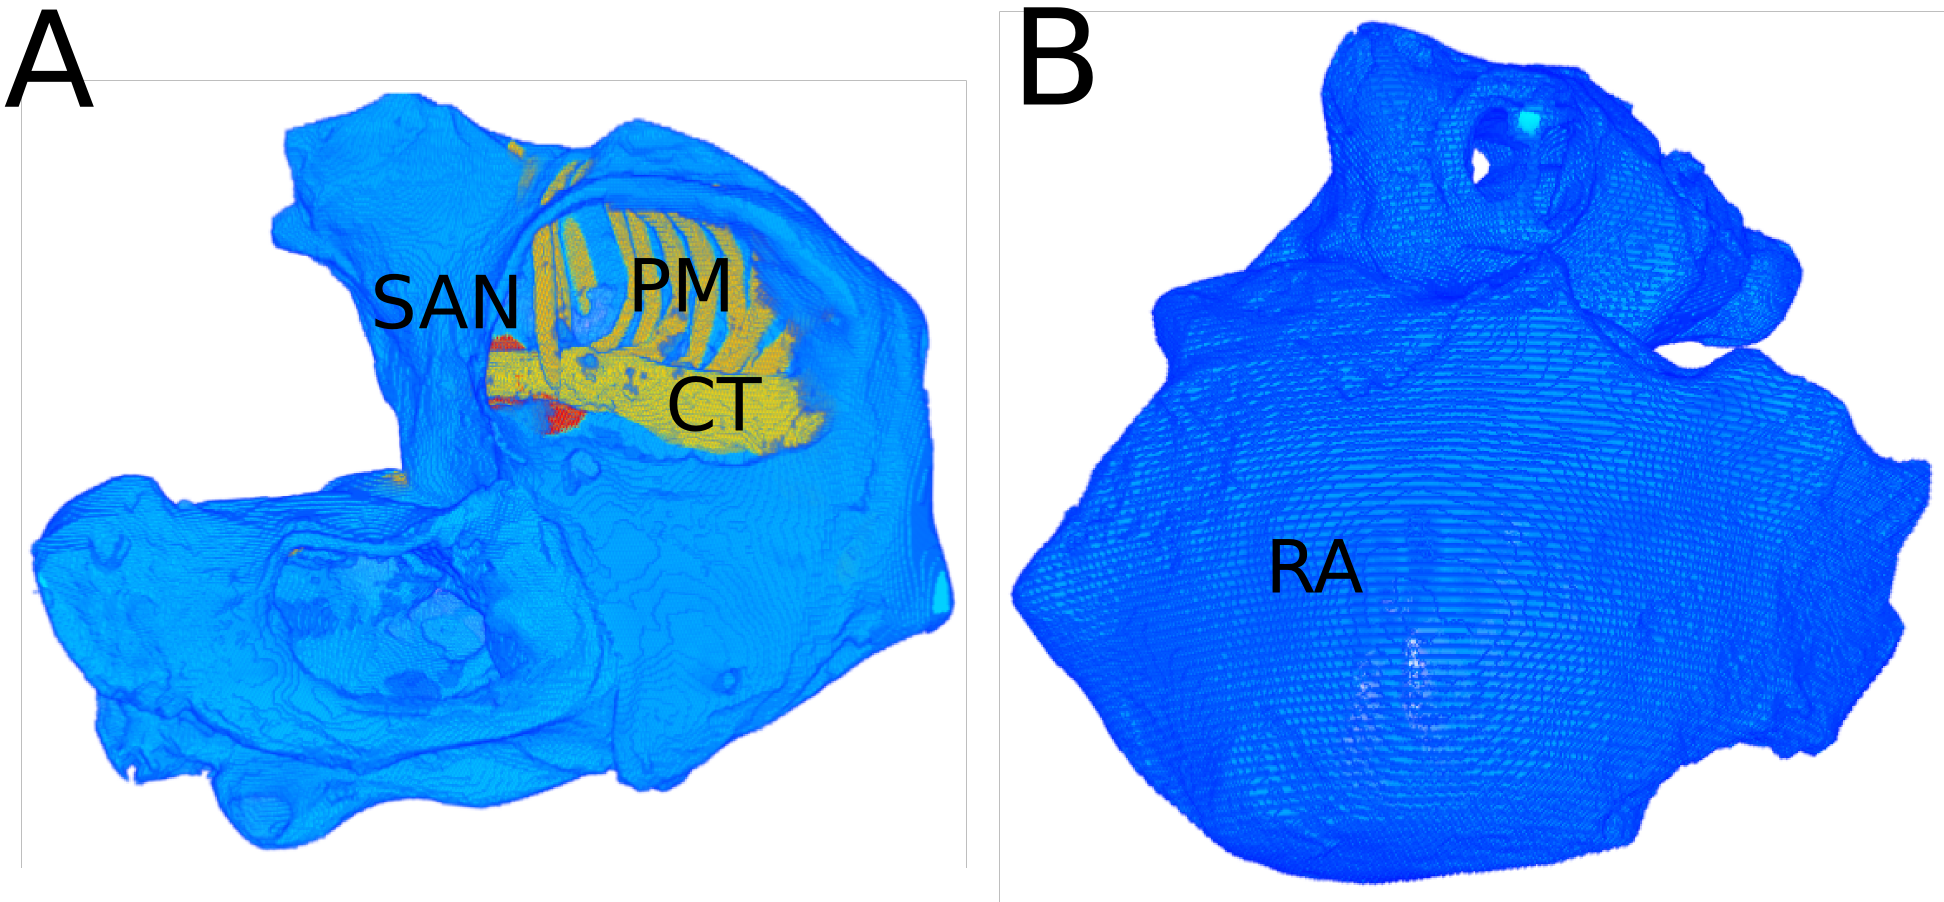
\includegraphics{figures/atrium/structure/atrial_geometry}
\caption[Atrial Geometry]{
\label{atrium:geometry}
(a)
View up into the right (RA) and left (LA) atria, showing the pectinate muscles
(PM, orange), crista terminalis (CT, yellow) and sino-atrial node (SAN, red).
The atrial muscle is shown in blue.
Also labelled are the right (RAA) and left (LAA) appendages.
(b)
A view of the atrial geometry looking down onto the wall of the right
atrium.  Visible at the top of the panel is the opening for one of the pulmonary
veins (PV).
}
\end{figure}

\begin{figure}
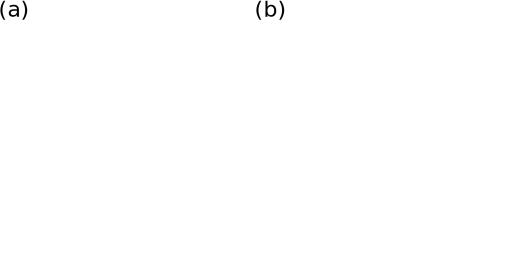
\includegraphics{figures/atrium/structure/fibres}
\caption[Atrial Fibre Structure]{
\label{atrium:fibres}
Representation of the fibre structure of the atrial geometry from a frontal
view (a) and a view up into the atria from the ventricles (b).
The arrows in red are aligned along the unit vectors of the fibre orientation.
The crista terminalis and the pectinate muscles are very easy to see with their
well defined fibre orientation.
}
\end{figure}

\section{Simulation Methods}
\label{atrium:sec:model}

\subsection{Atrial Model}

The electrical activity at each of the nodes was described by the equations of
the Courtemanche--Ramirez--Nattel (CRN) of the human atrial
myocyte~\cite{CRN98}.  This model, as previously described
($\S$\ref{sec:intro:math:crn}), is a second
generation model. It has 21 state variables, representing ionic gating activations
and inactivations and intracellular concentrations of ionic species.  In the
model, the total current, \ii{ion} is made up of the contributions of numerous
ion channels and exchangers.
\begin{align}
\label{atrium:crn}
\ii{ion} = \ii{Na} + \ii{K1} + \ii{to} + \ii{Kur} + \ii{Ks} + \ii{Kr} +
\ii{Ca,L} \nonumber \\
+ \ii{p,Ca} + \ii{NaK} + \ii{NaCa} + \ii{b,Na} + \ii{b,Ca}
\end{align}
where \ii{Na}, \ii{K1}, \ii{to}, \ii{Kur}, \ii{Ks}, \ii{Kr}, \ii{Ca,L},
\ii{p,Ca}, \ii{b,Na} and \ii{b,Ca}\ represent ionic currents and \ii{NaK}\ and
\ii{NaCa}\ are ion exchangers.  As a second generation model, the CRN model also
has a detailed calcium handling system which can influence the action potential
via its influence on the intracellular calcium concentration.

In some atrial simulations it was desirable to incorporate details of
electrophysiological heterogeneity to represent the regional difference in
electrical activity of atrial myocytes and the other cellular types present in
the geometry, such as the pectinate muscles and crista terminalis.
The parameters used for
heterogeneity were based on measurements taken by Feng et al.~\cite{Feng1998}
of the canine atrium.  These were converted to parameters for the CRN model by
Seemann et al.~\cite{Seemann2004} and have been used in several simulation
studies~\cite{Seemann2006,Stott2008}.  They are shown in
table~\ref{atrium:het_params}.

\begin{table}
\caption[Tissue Heterogeneity Parameters]{
\label{atrium:het_params}
Table showing the parameters altered to differentiate pectinate muscle (PM) and
crista terminalis (CT) cells, compared to the normal Courtemanche et al. (CRN)
parameters.
}
\begin{center}
\begin{tabular}{r c c c}
\toprule
 & CRN & PM & CT \\
\midrule
\g{to,max} & 0.1652 & 0.1652 & 0.2215 \\
\g{Ca,L,max} & 0.1238 & 0.1238 & 0.2067 \\
\g{Kr,max} & 0.0294 & 0.0294 & 0.0294 \\
\bottomrule
\end{tabular}
\end{center}
\end{table}

The CRN model was chosen for the biophysical detail it provides.
This enables the model to be used in the simulation of diseased or remodelled tissue, or
tissue under the influence of cardiac drugs.
The Fenton--Karma model, ($\S$\ref{sec:intro:math:fk}), is attractive as it is a
simpler model than the CRN model.
This makes it quick to simulate large timescale activity, but this same
simplicity can make incorporating drug actions or other behavioural
modifications difficult.
This made it inappropriate for use in many of the modelling studies the atrium
model would otherwise be useful for.


\subsection{Monodomain Equation}

To simulate the propagation of electrical activity over the finite difference
geometry previously described, the mono-domain equation
($\S$\ref{sec:intro:math:mono}) is used to describe the
changes in $V$ in time, $t$, the trans-membrane voltage.
\begin{equation}
\label{atrium:monodomain}
\frac{\partial V}{\partial t} = \nabla\cdot D \nabla V - \frac{\ii{ion}}{C_{m}}
\end{equation}
where $D$ is a tensor representing the diffusivity of electrical potential, \ii{ion} is described by the
CRN model (\ref{atrium:crn}), $C_{m}$ is the membrane capacitance and all other
symbols have their usual meanings.  Equation (\ref{atrium:monodomain}) is
advanced in time via the forward Euler method with a timestep of \ms{0.02}.  For
simulations with isotropic conductivity between nodes a 7-node approximation of
the differential operator is used.  When anisotropy is present, a 19-node
approximation is used.

The boundary conditions used in the simulation were the no-flux conditions.
A rule system based on the locations of nodes on the boundary was used to modify
the Laplacian to enforce the no-flux condition.
Nodes on the boundary had the differential of voltage set to 0 in the direction
of nodes outside the tissue~\cite{Aslanidi2009}.
This approximation was simple to implement.

\subsection{Tissue Anisotropy}

The heart has a complex fibrous structure (Chapter 1), and this manifests
electrically as regions which have preferential conduction directions.
The preferential conduction directions show greatly increased conduction
velocities, sometimes by a factor of up to five.
The fibre structure and regions of preferential conduction are generally
considered much more important for the ventricles than for the atria.
The atria, or more specifically the right atrium, do possess several structures
with a definite direction of preferential conduction.
These are the crista terminalis, responsible for rapid conduction of the
depolarization wave to the atrio-ventricular node, the pectinate muscles and the
Bachmann bundle, the preferential pathway for conduction between the atria.
To determine the influence of anisotropic conduction on the propagation of the
electrical activity, we follow a method after Panfilov and
Keener~\cite{Panfilov1995}.
In this method there is a unit vector, $\mathbf{f}$, defined at every point in
the tissue which has significant fibre orientation.
This unit vector defines a set of co-ordinate axes, in which the conductivity
tensor is diagonal
\begin{equation}
\label{atrium:dtilde}
\mathbf{\tilde{D}} =
\begin{pmatrix}
D_{\parallel} & 0 & 0\\
0 & D_{\perp} & 0\\
0 & 0 & D_{\perp}
\end{pmatrix}
\end{equation}
where $D_{\parallel}$ is the diffusion constant for conduction parallel to the
preferential direction of conduction and $D_{\perp}$ is the diffusion constant
for conduction perpendicular to this direction.
In this formulation it is assumed that there is no `sheet' structure which gives
a higher conduction velocity in one direction perpendicular to the main fibre
axis.
The diffusion tensor $\mathbf{\tilde{D}}$\ will only be diagonal in the
Cartesian co-ordinate system of the heart if the direction of preferential
conduction is parallel to one of the axes.
Therefore, to find the conductivity tensor in the global co-ordinate system,
$\mathbf{D}$, we need to find two transformation matrices $\mathbf{A}$\ and
$\mathbf{A^{T}}$\ such that
\begin{equation}
\label{atrium:d}
\mathbf{D} = \mathbf{A} \mathbf{\tilde{D}} \mathbf{A^{T}}
\end{equation}
To find $\mathbf{A}$\ it is possible to write out the involved rotations
explicitly, however an alternative method~\cite{Fenton2005}\ uses the fact that
$\mathbf{f}$\ and the two vectors orthogonal to it, $\mathbf{g}$\ and
$\mathbf{h}$\ are eigenvectors of $\mathbf{D}$.
These have the eigenvalues of $D_{\parallel}$\ and $D_{\perp}$.
The matrix $\mathbf{A}$\ is therefore an orthogonal matrix of the form
$\mathbf{A} = \left(\mathbf{f},\mathbf{g},\mathbf{h}\right)$ and so, using
(\ref{atrium:d}) $\mathbf{D}$\ can be written as
\begin{equation}
\label{atrium:dfgh}
\mathbf{D} = D_{\parallel}\mathbf{f}\mathbf{f^{T}} +
D_{\perp}\left(\mathbf{g}\mathbf{g^{T}} + \mathbf{h}\mathbf{h^{T}}\right)
\end{equation}
Using the fact that $\mathbf{A}\mathbf{A^T} = \mathbf{I}$ it is possible to
write
\begin{equation}
\label{atrium:dwithf}
\mathbf{D} = D_{\perp}\mathbf{I} + \left(D_{\parallel}-D_{\perp}\right)\mathbf{f}\mathbf{f^{T}}
\end{equation}
where $\mathbf{I}$\ is the identity matrix, and all other symbols are as defined
previously.
The directions of preferential conduction for the atrial geometry used in the
study were described by a pair of angles $\theta$ and $\phi$ representing the
orientation of the unit vector $\mathbf{f}$\ at each point in spherical polar
co-ordinates.
In cells with no assigned preferential conduction direction, the components of
$\mathbf{f}$\ were set to zero, giving a diffusion tensor of
\begin{equation}
\label{atrium:dnofibre}
\mathbf{D} =
\begin{pmatrix}
D_{\perp} & 0 & 0\\
0 & D_{\perp} & 0\\
0 & 0 & D_{\perp}
\end{pmatrix}
\end{equation}
which is the diffusion tensor for isotropic conduction.

The fibre orientations for the anatomical geometry used in this study are
defined in two files.
These two files contain the $\theta$ and $\phi$ components of the fibre vectors
between $0$ and $\pi$, discretised in 255 steps.
The relationship between the angles $\theta$ and $\phi$ and the unit vector of fibre
direction, $\mathbf{f}$, are shown in
figure~\ref{fig:atrium:structure:unit_vector}.
\begin{figure}
\begin{center}
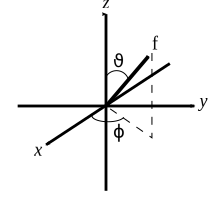
\includegraphics{figures/atrium/structure/unit_vector}
\end{center}
\caption[Relationship of $\theta$, $\phi$ and $\mathbf{f}$]{
\label{fig:atrium:structure:unit_vector}
The relationship of the angles $\theta$ and $\phi$ with the unit vector of fibre
orientation, $\mathbf{f}$.
The angle $\theta$ is the angle between the $z$ axis and $\mathbf{f}$.
The angle $\phi$ is the angle of rotation of $\mathbf{f}$ around the $z$ axis in
the $x\text{--}y$ plane.
}
\end{figure}
To convert $\theta$ and $\phi$ to the unit vector $\mathbf{f}$ we
use~\cite{Misner1973},
\begin{subequations}\label{eqn:atrium:structure:anglestof}
\begin{align}
f_x &= \cos\phi \sin\theta \label{eqn:atrium:structure:anglestofx}\\
f_y &= \sin\phi \sin\theta\label{eqn:atrium:structure:anglestofy}\\
f_z &= \cos\theta\label{eqn:atrium:structure:anglestofz}
\end{align}
\end{subequations}
where $\theta$ and $\phi$ are as indicated in
figure~\ref{fig:atrium:structure:unit_vector}\ and $f_x$, $f_y$, $f_z$ are the
$x$--, $y$--, $z$-- components of the vector $\mathbf{f}$.





\subsection{Computational Implementation}

The atrial geometry used in these studies is quite large, consisting of almost
19 million nodes.
As noted in \ref{atrium:sec:geometry}, only approximately 1.6 million of these
nodes correspond to active tissue--less than 10\% of the total.
The electrical activity at each node is represented by the CRN model and thus
requires 21 double precision numbers to be stored, representing the state
variables of the model.
The memory requirements of the model may be significantly reduced by storing
state variables, and where anisotropy is present the diffusion tensor, only for
the active nodes.
This reduces the memory requirements for storing the state variables from
approximately \unit{2.9}{GB}\ to \unit{256}{MB}.
A further simplification may be obtained by decomposing the geometry into a
linear array, containing the 6 or 18 neighbours of the active nodes to be used
in the diffusion tensor approximation.
The geometry and state information can therefore be represented by one linear
array of cellular states, one linear array used as a `map' and one
linear array representing the components of the Laplacian.
This linear data structure is very easy to parallelize on a shared memory
system.

The parallelization was accomplished through the use of the OpenMP shared
memory parallelism library~\cite{OpenMP}.
The system was then solved on 1 node of the Horace supercomputer on a total of 8
cores.
The linear array of active nodes was divided equally between the 8 cores, with
each core solving (\ref{atrium:crn}) for all nodes its assigned section of the
array.
A snapshot of the trans-membrane potentials at each of the active node sites was
output every \ms{1}\ of simulated time.
Simulation of \unit{1}{s}\ of atrial activity took 3.4 hours.
A parallel fraction between 0.98 and 0.99 was attained.

\section{Validation of the Model}

To verify the model, it was used to simulate a normal propagation, initiated
from the sino-atrial node.
The fully detailed model was used.
The Laplacian was precomputed to include all the information on tissue
anisotropy from the fibre orientation which accompanied the geometry.
The bulk diffusivity, $D$, of the tissue was set to $0.18\,\text{mm}^{\text{2}}\,\text{ms}^{\text{-1}}$.
This value was selected via numerical experimentation.
The parameter was adjusted until an appropriate activation time was attained.

The anisotropy ratio for transverse to longitudinal conduction was set to 1:9
after Seemann et al~\cite{Seemann2006}.
The activity at each node was represented by the Courtemanche et al. model with
voltage and ion concentration dependent parameters pre-computed and tabulated.
A timestep of \ms{0.02}\ was used to integrate both the cellular model at each
node and the diffusion of electrical activity between the nodes.
To initiate excitation a \unit{2}{nA}\ current was delivered for \ms{2} to cells
corresponding to the sino-atrial node of the model.
The excitation was then allowed to propagate without interference.
After the propagation was allowed to run its course, activation maps were
constructed.

The numerical implementation was within the theoretical limit of stability and
was tested by reducing the timestep to \ms{0.002}.
Whilst stimulating with this reduced timestep, a small ($>$5\%) difference in the relative number
of excited cells at any given timestep.
This difference was negligible compared to the total number of cells which could
be excited.
The solution was therefore considered to be stable.

\subsection{Activation Maps}

Snapshots of the electrical excitation are shown in
figure~\ref{fig:atrium:validation:main}\ and figure~\ref{fig:atrium:validation:valves}.
A map of activation times over the whole atria are shown in
figure~\ref{fig:atrium:validation:times}.
Excitation is initiated in the sino-atrial node.
The excitation wave is rapidly conducted along the muscle bundles which comprise
the crista terminalis and the pectinate muscles towards the base of the atrium
and the atrio-ventricular ring.
The influence of the preferential conduction along the crista terminalis and
pectinate muscle bundles is obvious on the epicardial surface of the right
atrium.
The presence of the muscle bundles on the endocardial surface causes earlier
activation of the epicardial surface.
The left atrium is activated first by the Bachmann bundle.
After this excitation spreads down and around the left atrial wall to the
atrio-ventricular ring and the left atrial appendage.
Complete activation of the right and left atria takes approximately \ms{120}.
After the activation there is an extended plateau phase, which lasts for
approximately \ms{100}.
During this plateau phase the whole atrium has a very uniform potential.
Repolarization begins at the sino-atrial node, following a very similar pattern
to the spread of excitation, with the region to first depolarise being that
which was first excited.
The repolarization appears to be less effected by the fibre structure of the
atrial model, with repolarized tissue spreading uniformly over the surface of
the right atrium.

\begin{figure}
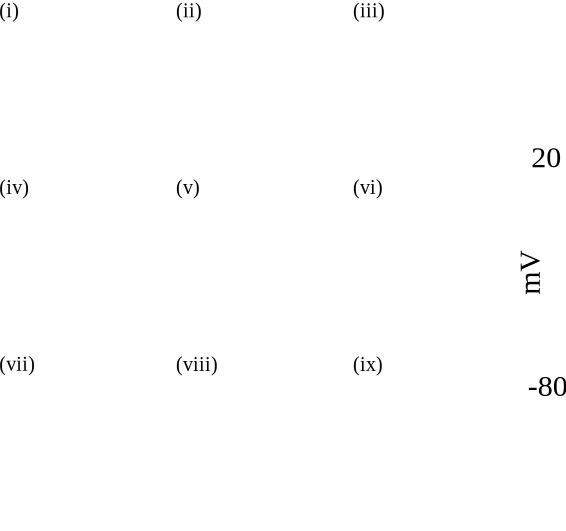
\includegraphics{figures/atrium/validation/front_activation}
\caption[Snapshots of Electrical Activation under Sinus Rhythm (frontal)]{
\label{fig:atrium:validation:main}
Simulated propagation of electrical excitation over the atrial model.
Excitation is initiated in the region corresponding to the sinus node.
Excitation spreads fastest along the fibres of the crista terminalis and the
pectinate muscles.
Snapshots shown for \ms{10}\ (i), \ms{15}\ (ii), \ms{20}\ (iii), \ms{25}\ (iv),
\ms{40}\ (v), \ms{60}\ (vi), \ms{180}\ (vii), \ms{200}\ (viii) and \ms{220}\ (ix).
}
\end{figure}

\begin{figure}
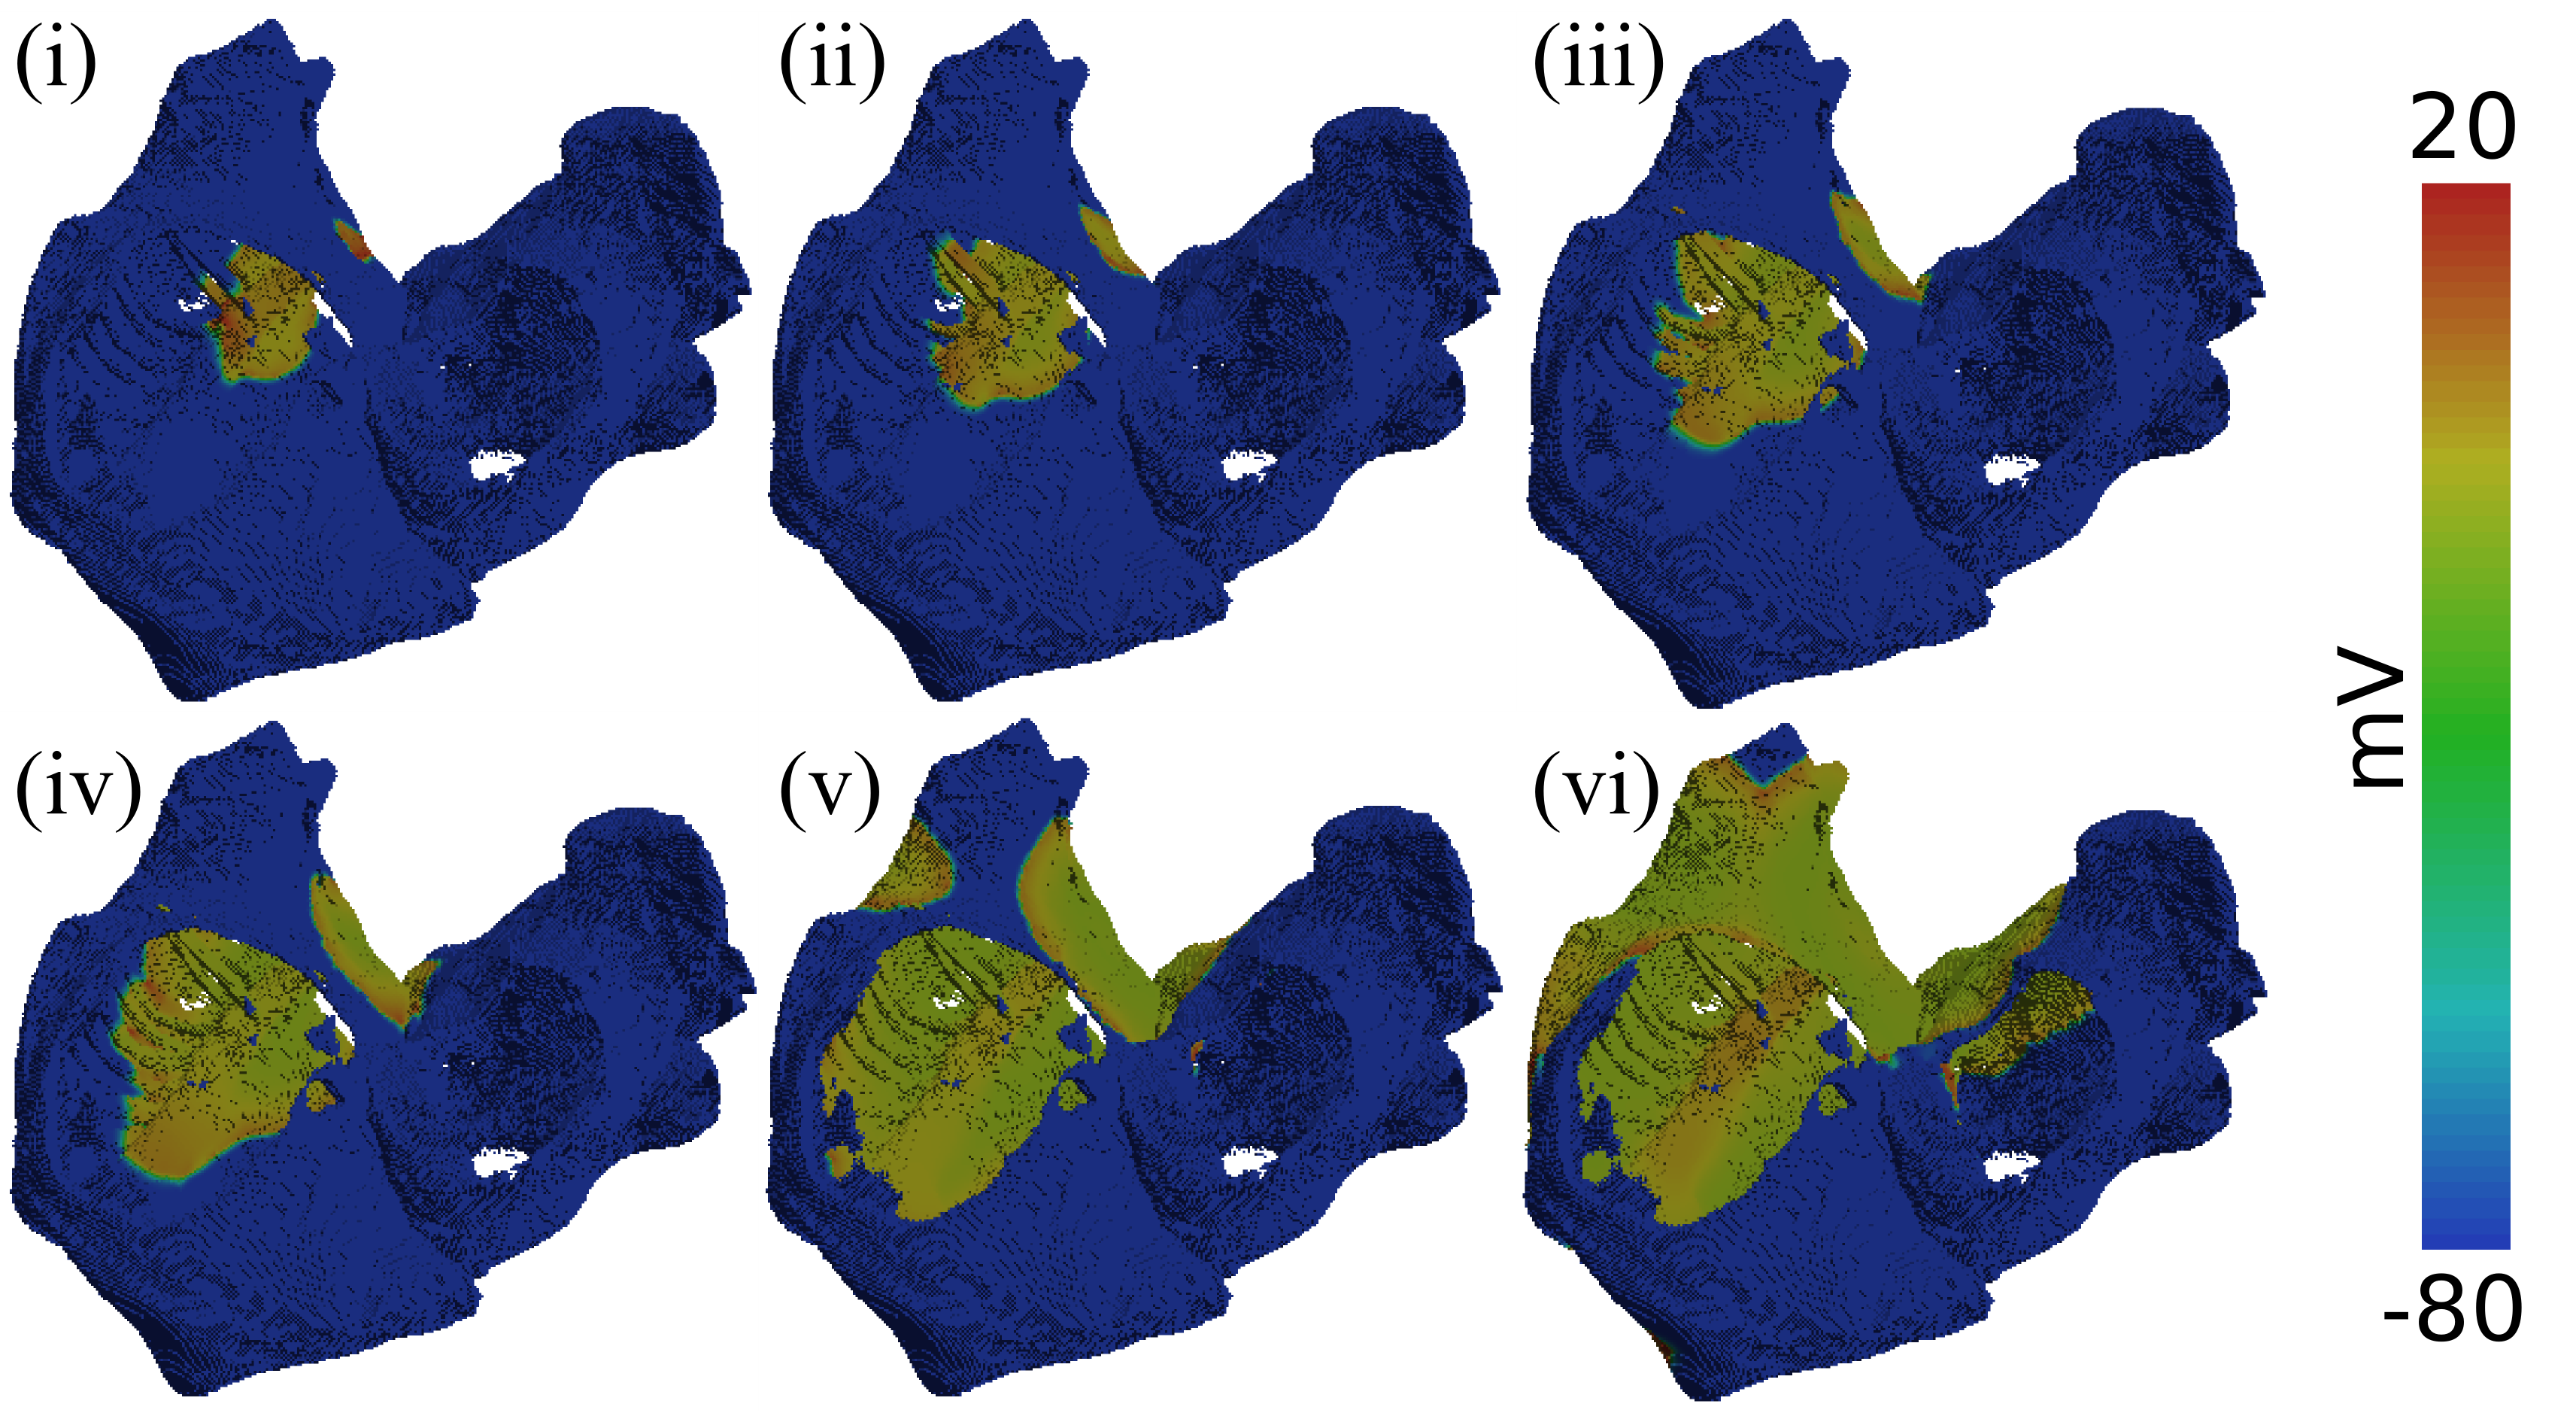
\includegraphics{figures/atrium/validation/back_activation}
\caption[Snapshots of Electrical Activation under Sinus Rhythm (from ventricular
openings)]{
\label{fig:atrium:validation:valves}
Simulated propagation of electrical excitation over the atrial model.
Excitation is initiated in the region corresponding to the sinus node.
Excitation spreads fastest along the fibres of the crista terminalis and the
pectinate muscles.
Snapshots shown for \ms{10}\ (i), \ms{15}\ (ii), \ms{20}\ (iii), \ms{25}\ (iv),
\ms{40}\ (v), \ms{60}\ (vi).
}
\end{figure}

\begin{figure}
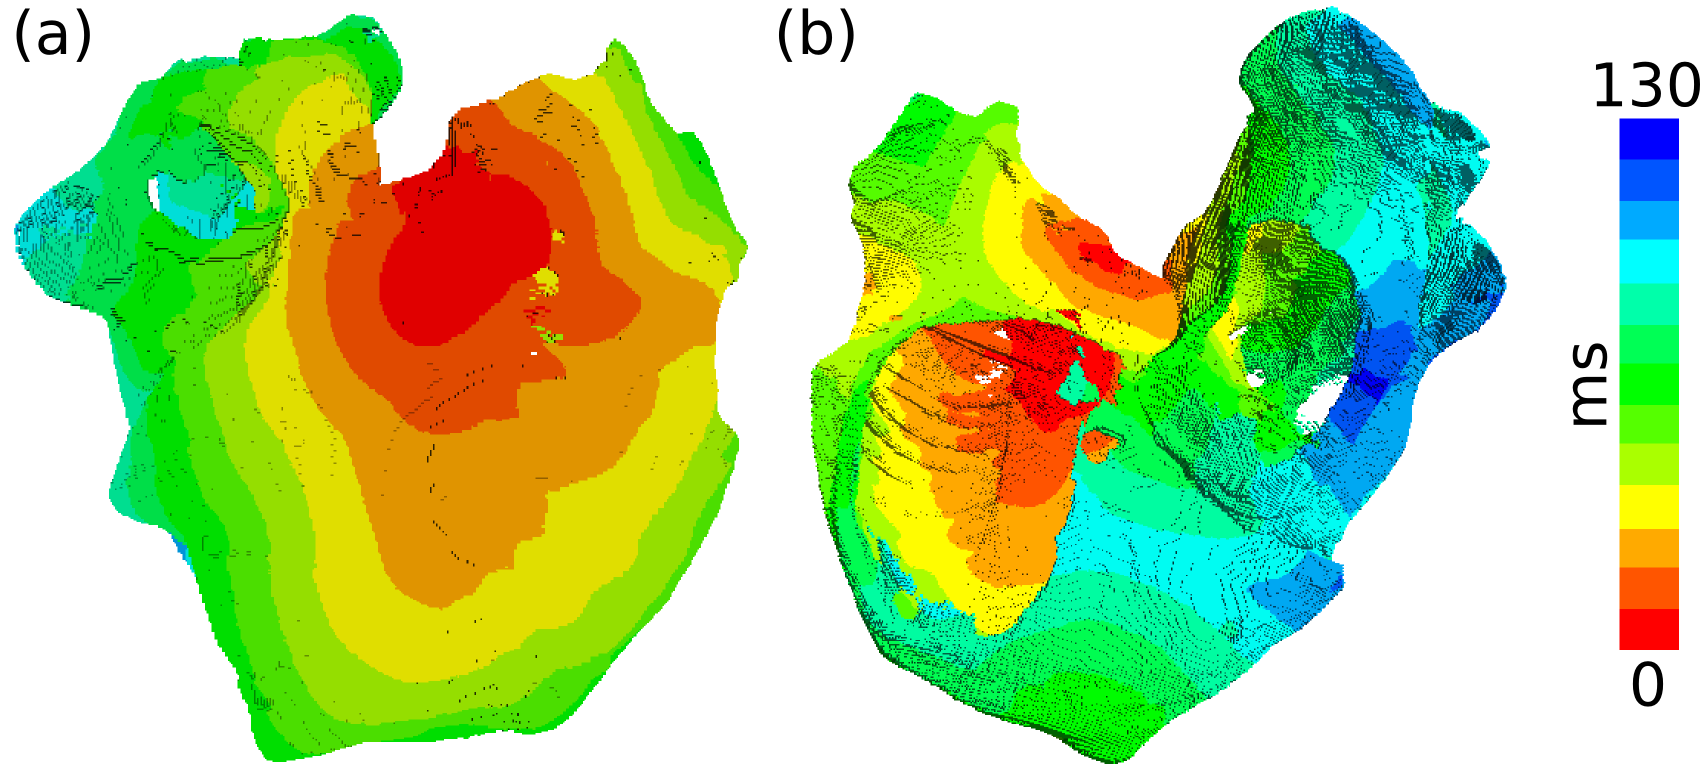
\includegraphics{figures/atrium/validation/activation_times}
\caption[Activation Times Under Sinus Rhythm]{
\label{fig:atrium:validation:times}
Activation times of the atrial geometry from a frontal view (a) and a
view from the ventricles up into the atria (b).
The influence of fibres on the activation times is clearly visible on both
views.
Excitation begins and the sinus node and spreads along the fibres over the
atrial epi- and endocardial surfaces.
The appendages are the last to activate.
}
\end{figure}

Once activated, the whole atrium takes \ms{121}\ to depolarise.
Time to depolarisation was taken as the time for a myocyte to attain a potential
of \mv{-60}.
The site of first activation of the endocardial surface of the left atrium
occurs at \ms{26}\ in the region of the Bachmann's bundle.
The time to total depolarisation of the endocardial surface was \ms{95}\ for
the right atrium and \ms{94}\ for the left atrium.
Conduction velocities were estimated from surface activation time information.
Conduction velocities are found to be $\text{1.30}\pm
0.05\,\text{ms}^{\text{-1}}$ in CT and $\text{0.75}\pm
0.06\,\text{ms}^{\text{-1}}$
in the atrial wall.


\subsection{Comparisons with Experimental Studies}

In a recent patient study Lemery et al.~\cite{Lemery2004} performed simultaneous recordings of
extracellular potentials on the endocardial surfaces of the atria of twenty
patients before they underwent catheter ablation therapy.
They found the total activation time under sinus rhythm for the endocardial
surfaces of both atria was \ms{120}.
The total activation time for the right and left atria was found to be \ms{81}\
and \ms{80}\ respectively.
The time to first activation of the left atrium at the Bachmann's bundle was
found to be \ms{41}.
The results from the simulated propagation are within the range of results
measured clinically for all times and within one SD of the mean for all
quantities except the left atrial activation time.

Conduction velocities for the classes of tissue present in the model have been
measured experimentally from $0.68\,\text{ms}^{\text{-1}}$ to
$1.03\,\text{ms}^{\text{-1}}$ for atrial wall
muscle~\cite{Hansson1998},
from $0.7\,\text{ms}^{\text{-1}}$ to 
$1.3\,\text{ms}^{\text{-1}}$ for crista
terminalis~\cite{Boineau1988} in the human atrium.
Conduction velocity in the pectinate muscles or Bachmann bundle has not been
measured experimentally in human studies.
The measured conduction velocities are within the experimental limits, providing
further confirmation.

\subsection{Comparisons with Existing Models}

There are several existing three dimensional models of conduction in the whole
human atrium~\cite{Harrild2000,Zemlin2000,Vigmond2001,Seemann2006}\ which use
some variant of a biophysical model for the atria.
Others, such as the cellular automaton approaches~\cite{Reumann2007} are not discussed here.
They represent a range of electrophysiological detail, fibre structure and
computational complexity.
The model of Harrild and Herenriqez~\cite{Harrild2000}\ has a detailed fibre
structure, but this is coupled with homogeneous electrophysiology.
In addition, the model has a relatively coarse space step, with an average
inter-element distance of \mm{0.55}.
The Zemlin~\cite{Zemlin2000}\ model was also based on the visible human dataset.
They used a reduced formulation of the Courtemanche et al. model which has 6
variables.
They included atrial wall muscle fibres based on dissection of anatomical
specimens.
There was no internal fibre structure such as the Bachmann bundle however.
It is a very efficient model.
The Vigmond~\cite{Vigmond2001}\ is an idealised model of an unusual construction.
It is topologically, rather than anatomically, correct and formulated as a
series of shells, made up of interconnected fibres.
The fibre based construction allows for efficient solutions.
The Seemann~\cite{Seemann2006}\ model is closely related to the model proposed in this
chapter--it would be accurate to say that this model is a simplification or
refinement of the Seemann model. 
The Seemann et al. model features an autoactive sino-atrial node complex, while
the model here focuses on the atrial conduction only.
It uses a full formulation of the Courtemanche et al model, without lookup
tables.
It features regions of differing bulk conductivity.
It is much more computationally demanding than the model proposed in this
chapter.

The model of the whole atrium proposed in this chapter represents a compromise
between electrophysiological detail and computational efficiency.
It includes differential electrophysiology and fibre orientation.
The omission of a functioning sino-atrial node is not a large flaw--many
pathological simulations involve non-physiological pacing protocols.
The additional incorporation of an MPI, rather than OpenMP, based implementation
would allow much more distributed execution, allowing long term simulations to
be performed.



\section{Mutation in KCNQ1: A Simulation Study}

Atrial Fibrillation (AF) is the most common arrhythmia in the developed world.
It is a self-promoting condition, with paroxysmal AF episodes frequently
degenerating into chronic and even permanent AF.
Clinically, AF patients show an erratic and high frequency ECG.
At the cellular level, AF is characterised by an abbreviated action potential
(AP) which has no plateau phase and poor heart rate adaptability.
The mechanisms through which AF influences the heart are complex, but the
remodelling of the cellular electrophysiology is believed to contribute to
reduced ERPs and through that, favour the formation of stable, long lived
spiral waves and organ level microwavelet re-entry.
AF is often preceded by congestive heart failure, cardiomegaly and other
structural cardiac diseases, but there are significant numbers of suffers with
no such structural defects.
There is also evidence of a genetic predisposition to AF, which is sometimes
termed Familial Atrial Fibrillation.
Several gene mutations have been causally implicated for AF, leading to AF
which manifests both with and without associated structural cardiac disorders.
The ion channels associated with the repolarization reserve (\ii{K1}, \ii{Kr},
\ii{Ks}) are particularly important to the genesis of AF.
Alterations in functions, gating and kinetics have been implicated in both short
and long QT syndromes.
The \ii{Ks}\ channel has very slow activation kinetics which enable it to
regulate cardiac APs over a wide range of plateau voltages.
Mutations in the \ii{Ks}\ channel are common.
Several mutations in the $\alpha$-subunit, coded for by the KCNQ1 gene, of the
\ii{Ks}\ channel have been identified including both loss-of-function and
gain-of-function, leading to the SQT syndrome and to AF.
Chen et al. studied a four generation Chinese family with hereditary persistent
AF.
They identified a missense mutation at nucleotide 418 from adenine to guanine
resulting in a change from serine to glycine at position 140 (S140G mutation of
\ii{Ks}).
This missense mutation lead to a large gain-of-function which included changes
in the channel kinetics.
It has been hypothesised that these changes in the function of the \ii{Ks}\
channel in the human atrium result in abbreviations of both APD and ERP and thus
provide an appropriate substrate for the genesis of AF.

This study had two goals: To construct a computer model of the available
experimental data from Chen et al. and to then use this model to quantify the
effects of the mutation through the use of cellular, 1D, 2D and 3D models.
From the data reported by Chen et al. it was expected that there would be a
significant alteration in channel kinetics needed to reproduce such traces.
In addition, any remodelling would need to sustain pacing at very high
frequencies.

\subsection{Methods}

\subsubsection{Modelling the Mutation}

This study, as in the previous chapter, uses the CRN model, developed by
Courtemanche et al.~\cite{CRN98}\ for simulation of the human atrial action
potential.
As a biophysically detailed model with 21 state variables and numerous ion
channels it is ideal for use in mutation studies.
The CRN model has individual descriptions of several $K^{+}$\ currents.
These include the time-independent potassium current, \ii{K1}, the ultra-rapid
potassium current, \ii{Kur}, the transient outward current, \ii{to}\ and the
rapid and slow delayed rectifier currents, \ii{Kr}\ and \ii{Ks}.
The latter current is modulated by the mutation and is described in the control
CRN cell by
\begin{equation}
\label{atrium:iks_con}
\ii{Ks} = g_{Ks}x_{s}^{2}\left(V-E_{K}\right)
\end{equation}
where $g_{\tiny{Ks}}$\ is the channel conductance (\unit{0.129}{nS/pF}), $x_{s}$\ is
the activation variable and $E_{K}$\ is the $K^{+}$\ reversal potential, found
through the Nernst potential.

\subsubsection{Simulation of the S140G mutation of KCNQ1 I-V relationship}

The Chen et al.~\cite{Chen2003} study determined that the most likely cause of
familial AF was was the S140G mutation of the KCQN1 gene, which forms part of
the $\alpha$-subunit of the \ii{Ks}\ channel.
The gene was transfected into COS7 cells along with the second component of
the $\alpha$-subunit, KCNE1, in both normal (WT) and mutated type (MT).
The transfected cells were used to perform voltage clamp experiments.
The clamp protocol used by Chen et al.~\cite{Chen2003} was as follows:
the cell was held at a holding potential of \mv{80} for \unit{0.5}{s}\ before
being held at \mv{10}\ steps between \mv{-130}\ to \mv{50}\ for \unit{3}{s}.
The voltage steps were followed by a \mv{-40}\ holding potential, applied for
\unit{1}{s}.
The values of \ii{Ks} at the end of the step voltages were plotted against the
step voltages to determine  I-V relationships for WT
and MT cells, shown in figure~\ref{atrium:iks:vc}(a) (points with errors) and
current traces, shown in figure~\ref{atrium:iks:vc}(b) and (d) for WT and MT,
respectively.

\begin{figure}
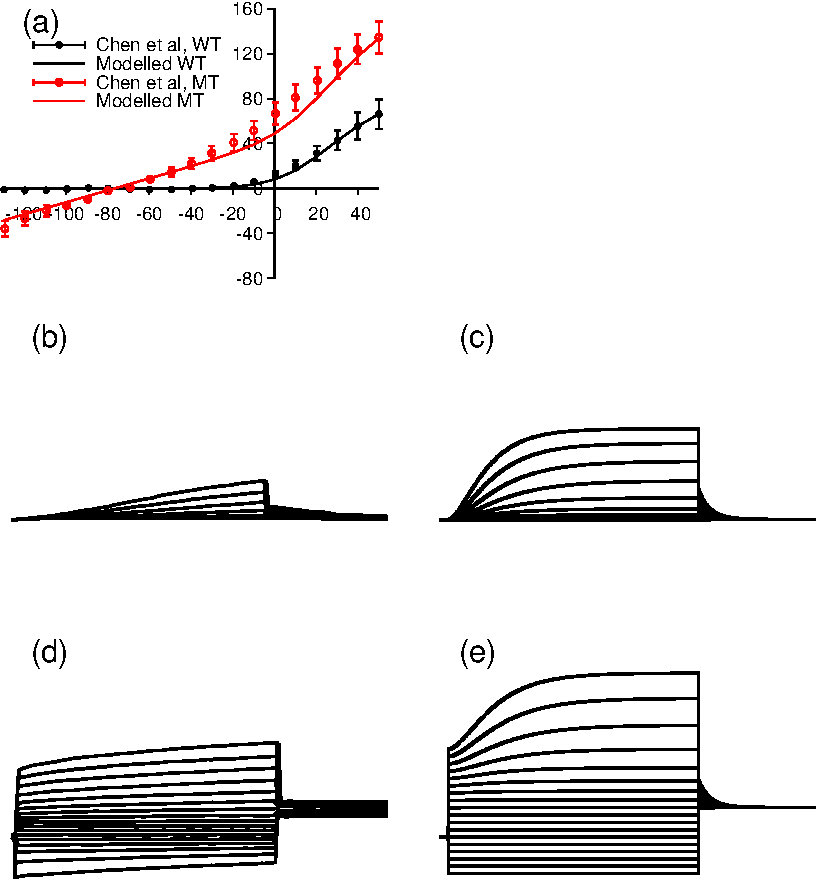
\includegraphics{figures/atrium/iks/figures/01_IV}
\caption[KCNQ1 mutation in IKs, experimental data]{
\label{atrium:iks:vc}
(a) Experimental WT (black, closed circles) and MT (red, open circles)
I-V relationships recorded by Chen et al~\cite{Chen2003}.  Simulated I-V curves for WT (black
lines) and MT (red lines).  Modelled curves are scaled to experimental points
based on the WT current density at \mv{50}.
(b) Experimental current traces for WT.
(c) Simulated current traces for WT.
(d) Experimental current traces for MT.  Note the instantaneous
activation, and the significant inward current at negative clamp potentials.
(e) Simulated current traces for MT.
}
\end{figure}

The I-V relationship shows that the mutation causes a gain-of-function across
all the clamp potentials.
It also reveals that the mutation appears to cause an inward current at negative
potentials.
The current traces suggest a drastic change in the kinetics of the \ii{Ks}\
channel with a significant component of the current being activated immediately.
The addition of a leakage component to (\ref{atrium:iks_con}) allowed simulation
of \ii{Ks}\ characteristics which closely matched the experimental data.
Under MT conditions, the new total current \iip{Ks}\ was described by
\begin{equation}
\label{atrium:iks_mut}
\iip{Ks} = \ii{Ks} + \varphi g_{Ks}x\left(V-E_{rev}\right)
\end{equation}
where \ii{Ks}\ is (\ref{atrium:iks_con}), $\varphi$\ is a multiplicative parameter
from with values between 0 and 1, $g_{Ks}$ is as in (\ref{atrium:iks_con}) and
$E_{rev}$\ is the reversal potential of the leakage component.
The reversal potential was estimated from the experimental I-V relationships to be
\mv{-76.3}.
The inclusion of the $\varphi$\ parameter allowed the simulation of several
intermediate mutant states, representative of a heterozygous mutation.
Setting $\varphi = 1$\ and following the voltage clamp protocol the I-V relationship of \ii{Ks}\ was simulated to
provide a good match to experimental data, shown as the lines in panel (a) of
figure~\ref{atrium:iks:vc}.
Also shown are the simulated current traces elicited by the voltage clamp
protocol in panels (c) and (e).
The non-gated leakage component of \iip{Ks}\ sufficiently accounts for the
changed current density and kinetics.
Note that in panel (a) the modelled current traces have been normalised by the
maximum current observed with a normal \ii{Ks}\ and the WT KCNQ1.
The differing time-course of the currents are likely due to the different temperatures
at which the simulations were performed.
However, no data on the temperature dependence of \ii{Ks}\ was available.

\subsubsection{Simulation Protocols}
\label{sec:atrium:s140g:methods}
To assess the effects of the mutation on human atrial myocytes, cellular models
including the modified \iip{Ks}\ described by (\ref{atrium:iks_mut}) were used
in a number of simulation protocols, as described in Chapter 2.
Initially the \apd\ was evaluated under conditions corresponding to $\varphi =
0$\ (WT) and $\varphi = 1$\ (MT).
Under such conditions, the induced \apd\ shortening was found to result in
un-physiological \apd\ values, shown in figure \ref{atrium:iks:apd}.
Therefore a pair of heterozygous cases, corresponding to $\varphi = 0.10$\
(HT10) and $\varphi = 0.25$\ (HT25) were created and used in the evaluation of
the mutation's effects.

Using the models and protocols described in Chapter 2 the \apdr, ERP\emph{r}, VW,
CV\emph{r}, SVW and the dynamic behaviours of spiral waves were evaluated for
the WT, HT10 and HT25 cases.
For the 3D simulations, the model described in Sections
\ref{atrium:sec:geometry}\ and \ref{atrium:sec:model}\ was used.

The diffusion coefficient, $D$, was set to
$0.03125\,\text{mm}^{\text{2}}\,\text{ms}^{\text{-1}}$~\cite{Biktasheva2005}\
for all tissue simulations.
This is lower than the value used for the atrium model in the previous section.
The reduced value allows scroll waves to be initiated easily in both control and
mutant conditions.
A reduction of intracellular coupling has been noted in experimental and
clinical studies of atrial fibrillation~\cite{Velden1998,Shaw1997}.

The Dominant Frequency (DF) of the tissue activity in 2D cases was estimated
using a Fast Fourier Transform~\cite{Zaitsev2000}\ (FFT) to compute the power
spectrum.
Voltage traces from selected points through the diagonal were used as the input.
Matlab was used to compute the FFT.
The \unit{10}{s}\ duration of the simulation gives a resolution of
\unit{0.1}{Hz}.
Ascertaining the DF from the FFT reveals the primary frequency of activation of any
source in the tissue, with multiple sources revealed as multiple peaks.
Conversely, if there is no coherent source, the power spectrum will lack clear
peaks.
An alternative might have been to use a threshold crossing
algorithm~\cite{Chen1996}.
These are more commonly applied to ECG recordings.
In such an algorithm the time interval between instants the voltage signal crosses
a particular threshold, typically 20\% of the maximum, in a given window,
typically \unit{1}{s}, is recorded.
From the average of such intervals, the rate can be estimated.
The evolution of the rate can also be tracked, from interval to interval.
Using a threshold crossing interval method has some advantages over the FFT
based approach chosen, since it hard to track the evolution of rate with an FFT
algorithm.
However, if desired, zero padding could be used to estimate the DF for
each \unit{1}{s}\ segment with an FFT.
The use of an FFT makes multiple sources clearer than a threshold crossing
interval, as there will be two peaks, instead of high variability in
interval.


Since the intention was just to investigate the influence of the mutation, the
model was used without tissue anisotropy.
The mutation was applied homogeneously with the electrical activity at all
nodes described by either the WT or HT25 cells.
There was no heterogeneity introduced to account for the differing cell types
present in the human atrium.
To examine the behaviour of scroll waves under WT and HT25 conditions a protocol
analogous to the wave-break protocol described for 2D sheets of tissue was
used~\cite{Kharche2007}.
The protocol is illustrated in figure~\ref{atrium:iks:scroll_init}.
\begin{figure}
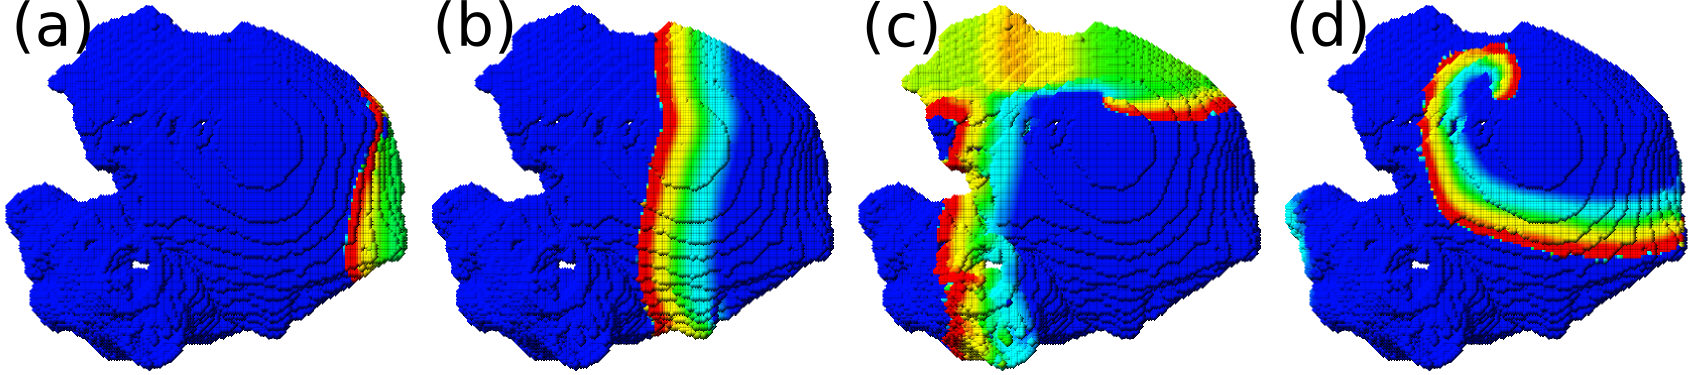
\includegraphics{figures/atrium/iks/scrollhowto}
\caption[Initiating a Scroll Wave]{
\label{atrium:iks:scroll_init}
Stimulus protocol used to initiate a scroll wave.
(a) One extreme of the atrial model is stimulated
(b) The excitation is allowed to propagate
(c) An S2 stimulus is delivered by clamping a section of the tissue, here
the upper quarter.
(d) A scroll wave begins on the wall of the right atrium.

NB: The shorter action potential shown in this figure was selected for clarity.
It is very short when compared with figure~\ref{fig:atrium:validation:main}.
This is due to a combination of the reduced value of $D$ used in this study and
the shortening of the action potential induced by the mutation under study.
}
\end{figure}
First, a small number of cells are simulated at one extreme of the atrial model.
The excitation is allowed to propagate through the model until the S2 stimulus
is delivered.
The S2 stimulus is delivered via briefly clamping a section of the atrial model to
\mv{50}\ and then releasing the clamp.
A correctly timed S2 stimulus results in a scroll wave on the wall of the right
atrium.
After initiation, the models were simulated until activity ceased or until
\unit{6}{s}\ of simulated time had elapsed.

\subsection{Results}

\subsubsection{Changes in \apd\ due to S140G mutation}

The effect of an increase in the leakage current parameter were investigated.
This was done using the standard \apd\ protocol and varying $\varphi$\ between
0 and 1.
Variation in \apd\ as $\varphi$\ is altered is shown in
figure~\ref{atrium:iks:apd}(a).
Representative APs are shown in figure~\ref{atrium:iks:apd}(b).
The \apd\ under Control conditions (WT) was seen to be \ms{312.0}.
Progressive mutation decreased the \apd\ to \ms{150.5}\ in HT10 case and
\ms{79.3}\ in HT25 case.
Under homozygous conditions, $\varphi = 1$\, the \apd\ was seen to be \ms{22.4}.
Figure~\ref{atrium:iks:apd}(b) shows the inclusion of the mutant channel causes
the changes in morphology associated with none of the mutant types having a
plateau region.
Inclusion of the mutant channel decreased the upstroke velocity of the AP from
\unit{217.1}{V/s}\ in WT, to \unit{214.0}{V/s}\ in HT10 and \unit{208.6}{V/s}\
in HT25.
The upstroke velocity in the homozygous case was \unit{192.0}{V/s}.
\begin{figure}
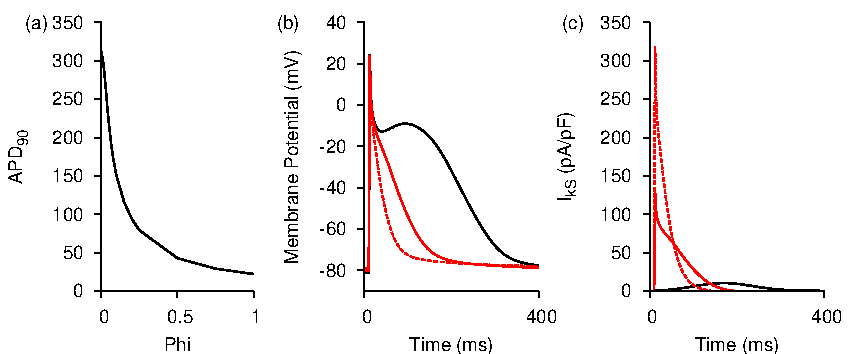
\includegraphics{figures/atrium/iks/figures/02_APD}
\caption[AP and current profiles with S140G mutation]{
\label{atrium:iks:apd}
(a) Plot of \apd\ vs $\varphi$, showing how increasing mutation reduces \apd.
AP profiles (a) and \ii{Ks}\ current profiles (b) for WT (black), HT10 (red,
solid) and HT25 (red, dashed).
Stimulus is delivered at \ms{10}.
Note the large increase in current density under the S140G mutation, which
causes a corresponding flattening of the AP profiles and removal of the plateau.
}
\end{figure}
Figure~\ref{atrium:iks:apd}(c) shows the current profiles of \ii{Ks} over the course of
an AP which correspond to the AP traces shown in panel B.
\ii{Ks}\ is seen to increase considerably in both the HT10 and HT25 cases
compared with the WT case.
The leak also changes the morphology of the current profile to one showing
almost instant activation in HT10 and HT25 cases, compared to the slow
activation in WT.

\subsubsection{\apdr\, ERP\emph{r}, CV\emph{r} and VW}

\begin{figure}
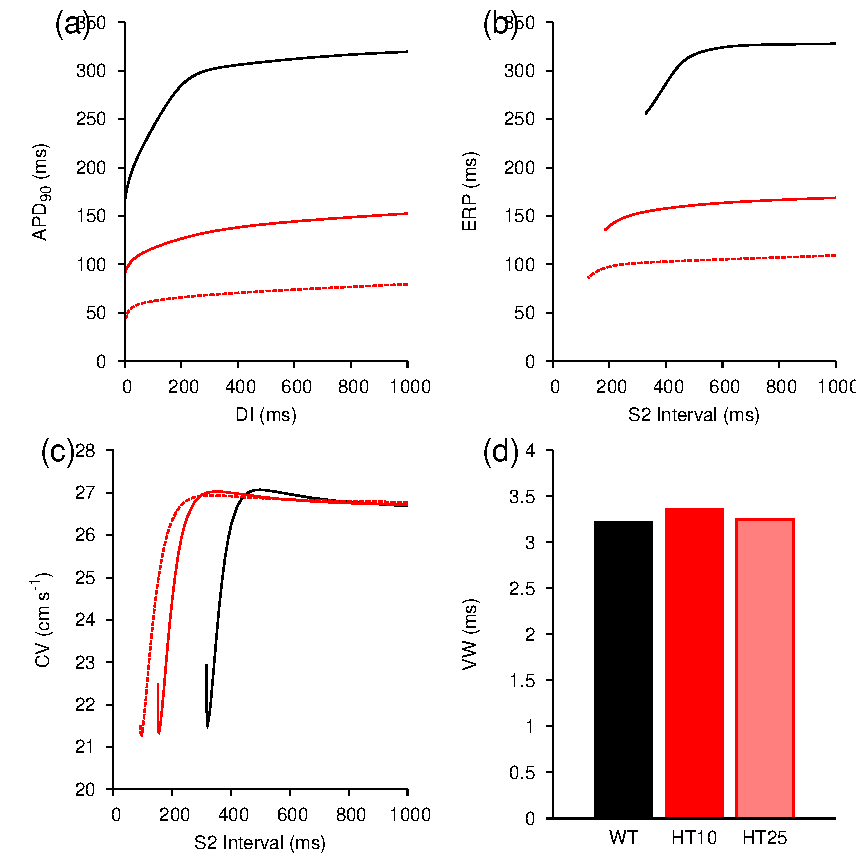
\includegraphics{figures/atrium/iks/figures/03_REST}
\caption[Restitution properties with S140G mutation]{
\label{atrium:iks:apdretal}
Restitution curves for WT (black), HT10 (red, solid) and HT25 (red, dashed).
(a) \apdr.
(b) ERP\emph{r}.
(c) CV\emph{r}.
(d) Temporal VW to premature stimulus.
}
\end{figure}

The \apdr\, figure~\ref{atrium:iks:apdretal}(a), reflects the decreased \apd\ with
the restitution curves considerably flattened for both the mutant cases.
The ERP\emph{r}\ curves, figure~\ref{atrium:iks:apdretal}(b), also reflect the
reduced \apd\ and show a similar flattening to that seen in the \apdr\ curves.
At an S1 interval of \ms{1000}\ the ERP was found to be \ms{327.2}\ in WT,
\ms{168.4} in HT10 and \ms{109.3} in HT25.
In addition, the mutant cases supported excitation at much lower S1 intervals
(or higher pacing rate) compared to the control case.
The minimum S1 interval sustained during the ERP\emph{r}\ calculations was
\ms{328.7}\ in WT, \ms{184.3} in HT10 and \ms{126.7} in HT25.
The solitary wave CV was not altered considerably by the mutation (\cms{26.7}\
in WT c.f. \cms{26.8} in HT25).
The CV\emph{r}\, figure~\ref{atrium:iks:apdretal}(c), curves confirm the findings
of the ERP\emph{r}\ calculations, that the mutant case supports successful
excitation after a considerably reduced S2 interval.
The minimum S2 interval which still allowed the test stimulus to propagate was
found to be \ms{317.1}\ in WT, \ms{151.7}\ in HT10 and \ms{92.5}\ in HT25.
Vulnerability to premature excitation was relatively unaffected by the mutation.
It was observed to increase in tissues where the mutation was present from a VW of
\ms{3.2}\ in WT to \ms{3.4}\ in HT10 and \ms{3.3}\ in HT25
(figure~\ref{atrium:iks:apdretal}(d)).
This is a small (less than 5~\%) change in the VW to premature excitation.

\subsubsection{Dynamic Behaviours on a 2D sheet}

Re-entry was initiated in 2D sheets of homogeneous virtual human atrial tissues
for WT, HT10 and HT25 cases.
The dynamical behaviours of the system were observed for \unit{10}{s}\ or until
all electrical activity ceased after the re-entry self terminated.
Frames from the simulation and spiral tip traces are shown in
figure~\ref{atrium:iks:twodframes}.
The lifespan of re-entrant waves in the WT case was seen to be \unit{2.8}{s},
whilst in both the HT10 and HT25 cases the re-entry persisted for the duration
of the simulation (\unit{10}{s}).
In the WT case the spiral tip showed a large degree of meander
(figure~\ref{atrium:iks:twodframes},top row, column iv) even after the initial
transitory period.
The tip trajectory shows that the spiral wave completes several rotations, each
accompanied by large movements of the tip before finally tip exits along the
lower edge of the tissue, unable to move back into the tissue due to its own
refractory tail.
In contrast in both HT10 and HT25 cases the meander is confined to a relatively
small area after after the initial transitory period.
The spiral wave tip precesses around a stationary point in a flower petal
pattern, indicative of a highly stable re-entrant wave.

\begin{figure}
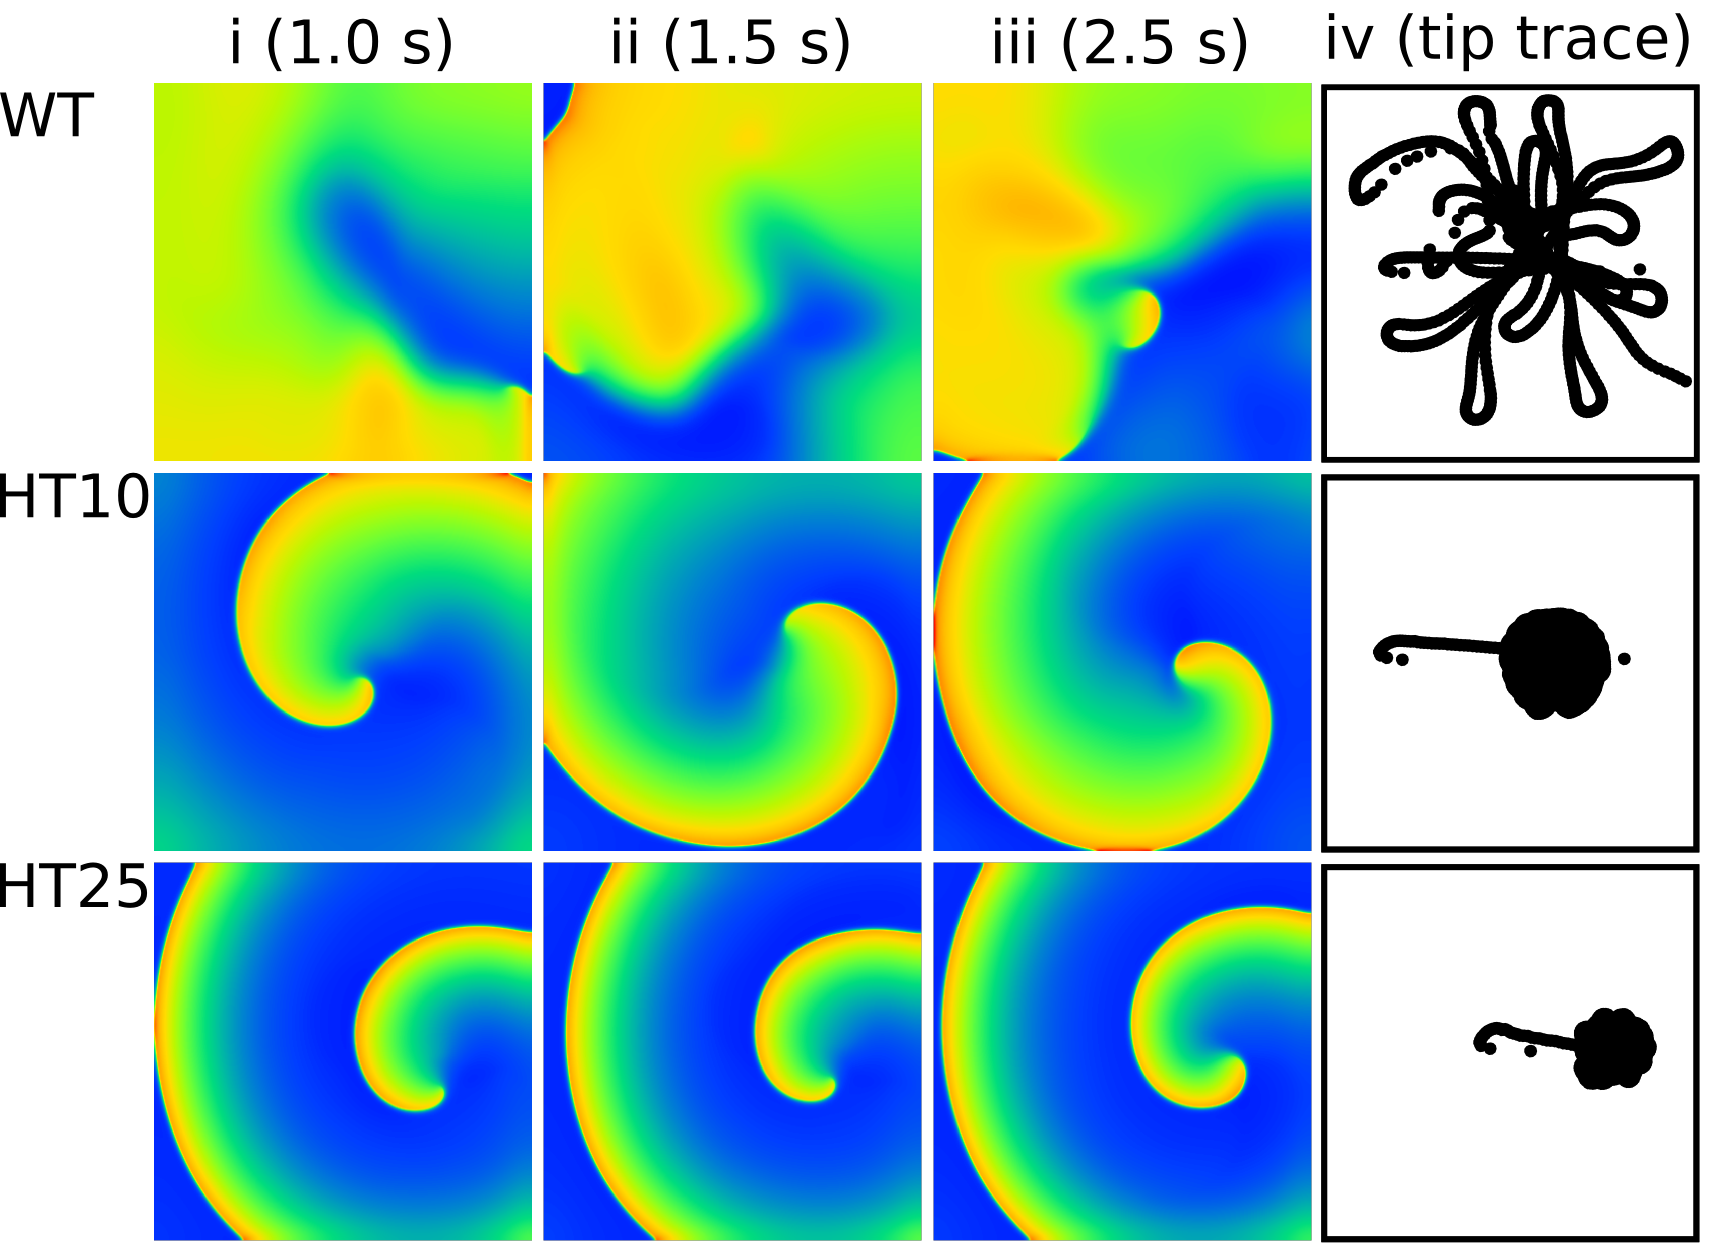
\includegraphics{figures/atrium/iks/2Dplots}
\caption[2D Re-entry under S140G conditions]{
\label{atrium:iks:twodframes}
Snapshots of electrical activity extracted at \unit{1}{s}\ (i), \unit{1.5}{s}\
(ii) and \unit{2.5}{s}\ (iii) after spiral wave initiation, with accompanying
tip trace shown in (IV) for WT (top), HT10 (middle) and HT25 (bottom).  In the
electrical activity plots red is fully depolarized, blue is the resting
potential.  The WT spiral occupies much more of the tissue and has a very large
meander, compared with the HT10 and HT25 cases, which show a very stable spiral
after the initial transient behaviour.
}
\end{figure}

Representative APs were extracted from a point in the tissue and used in
dominant frequency analysis, shown in figure~\ref{atrium:iks:twodfreq}.
From the representative APs (top panels) it can be seen that the \apd\ decreases
as a greater proportion of the mutation is present.
The WT case also shows obvious alternans in the AP profiles reflecting its
unstable and meandering spiral wave, contrasting with the general uniform APs
seen with the HT10 and HT25 cases.
Dominant frequency analysis of AP profiles (bottom panels) extracted along the
sheet diagonal was performed.
The dominant frequency analysis shows that whilst in the WT case there is a
relatively low frequency of oscillations (less than \unit{4}{Hz}) compared with
the mutant cases (\unit{7}{Hz} in HT10, \unit{10}{Hz} in HT25).
The width of the peaks for the two mutant cases are smaller, indicating a
greater stability compared to the more dispersed frequencies seen in the WT
case.

\begin{figure}
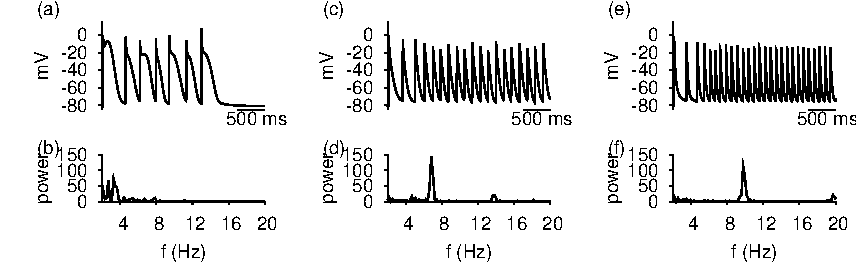
\includegraphics{figures/atrium/iks/figures/05_2D_freq}
\caption[Frequency of extracted APs from 2D sheets with S140G mutation]{
\label{atrium:iks:twodfreq}
Representative AP traces (top panels) and dominant frequency analysis (bottom
panels) for WT (left), HT10 (centre) and HT25 (right).  Traces extracted from a
point \mm{6}\ from top and left of the 2D sheets every \ms{2.5} of elapsed time.
}
\end{figure}

The minimal stimulus substrate size was computed as shown in
figure~\ref{atrium:iks:svw}.
The mutation induced remodelling dramatically reduced the size of the SVW, from
\mm{99.1}\ in WT conditions to \mm{12.3}\ in HT25 conditions, a reduction of
87.5\%.

\begin{figure}
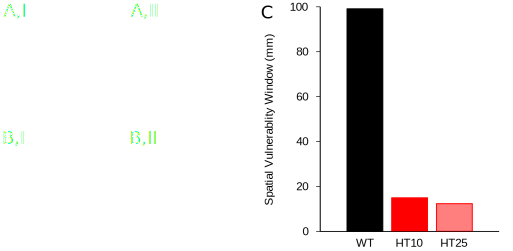
\includegraphics{figures/atrium/iks/07_svw}
\caption[Spatial Vulnerability Window with S140G mutation]{
\label{atrium:iks:svw}
(a) Unsuccessful attempt at initiating figure-of-eight re-entry just
before (I) and after (II) re-entry would occur.
(b) Successful initiation of figure-of-eight re-entry just before (I) and
just after (II) re-entry is initiated.
(c) Spatial vulnerability window for WT (black), HT10 (red) and HT25
(pink) tissue.
Spatial vulnerability window is the minimum length of tissue that produces
figure-of-eight re-entry.
}
\end{figure}

\subsubsection{Modelling the S140G mutation in the Whole Atrium}

Scroll waves were initiated in the whole atrial model as described in
\ref{sec:atrium:s140g:methods}.
Scroll wave behaviour for control (WT) and $\varphi = 0.25$\ (HT25) were studied
as representative cases.
The scroll waves were initiated on the right atrial free wall to allow
initiation and initial evolution without interference with anatomical obstacles.
The 3D simulation visualisations are presented in
figure~\ref{atrium:iks:threed}.
In WT conditions, as observed in the 2D simulations, the scroll waves have a
large meander and self-terminated in approximately \unit{4.2}{s}.
As long as the scroll wave was initiated far from anatomical obstacles such as
venous openings, self-termination was independent of position.
In certain cases where it was not `entrapment' of the scroll wave around an
anatomical obstacle was observed, leading to prolonged scroll wave activity even
in the WT case.
Under HT25 conditions the small wavelength allowed scroll waves to become
persistent in all cases, as observed in 2D simulations.
In contrast to the 2D simulations the presence of anatomical obstacles led to break up of the
scroll wave into erratic propagations and short-lived wavelets.
This erratic behaviour then persisted until the end of simulation at
\unit{6}{s}.

\begin{figure}
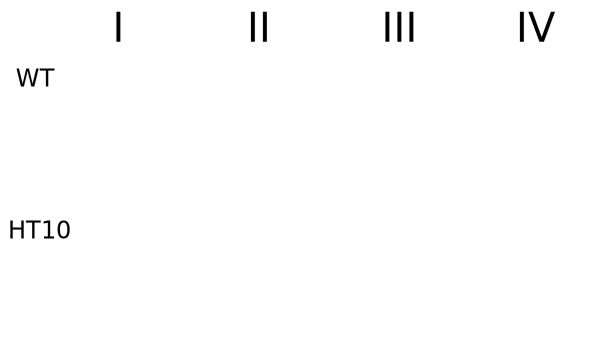
\includegraphics{figures/atrium/iks/3D_Fig}
\caption[Snapshots of membrane potential over the whole atrium with S140G
mutation]{
\label{atrium:iks:threed}
Snapshots of the membrane potential for WT (top panels) and HT25 (bottom
panels) taken at \unit{1}{s} (i), \unit{2}{s} (ii), \unit{3}{s} (iii) and
\unit{4}{s} (iv) of simulated time.
In the plots, red shows full depolarized tissue, whilst blue tissue is at rest.
By \unit{2}{s} the activity shown in panel bottom,ii has started to break up, compared with
the more stable ave shown in the upper panel, just about to self-terminate in
panel top,iv, as the excitation wavefront hits the non-conducting atrio-ventricular
ring.
}
\end{figure}

Representative AP profiles were extracted from several points throughout the
atrial model and used in dominant frequency analysis.
The dominant frequency in the HT25 case was found to be much higher,
approximately \unit{10}{Hz}, than in the WT case, less than \unit{3}{Hz}.
%This is shown in figure~\ref{atrium:iks:threeddf}.

\subsection{Discussion and Conclusions}

The S140G mutation of the KCNQ1 $\beta$\ subunit of the \ii{Ks}\ ion channel
causes a large gain of function.
This gain of function manifests as a component of the \ii{Ks}\ channel which
shows instantaneous activation kinetics under voltage clamp conditions.
Modelling the effects of the mutation as the addition of a leakage component
with constant conductance to the \ii{Ks}\ channel therefore seems to be a good
fit to the experimental data provided by Chen et al.
Incorporation of the mutation into models of cellular electrophysiology
dramatically reduces the \apd\ and the ERP.
The increased repolarization current also flattens the plateau region, or
eliminates it entirely.
Conduction velocity was not significantly affected by the presence of the
mutation, possibly due to the leakage component being inward at resting
potentials, contributing to the upstroke.
In 2D simulations, the mutation stabilised re-entrant spiral waves, leading to
long lived arrhythmic activity at a high frequency.
In 3D, simulations showed that with the addition of anatomical obstacles,
scroll-waves would instead break up.
The shorter wavelength and refractory length introduced by the mutation assists
in the maintenance of the fibrillatory activity.
The fibrillatory activity in the presence of the mutation shows a very high
frequency, approximately \unit{600}{bpm}, which is in agreement with the
definition Chen et al. used when selecting AF sufferers for their study.
The Chen et al. hypothesis is supported by this study, which reproduces both
voltage clamp experiments and then provides insight into the mechanisms
responsible for the maintenance of AF in those afflicted with the mutation.

Repolarisation of cardiac myocytes depends on the \ii{Ks}\ (KCNQ1/KCNE1) and
\ii{Kr}\ (hERG) channels.
Previous clinical and simulation studies have linked mutation leading to
gain of function in the \ii{Ks}\ to SQT syndromes~\cite{Brugada2004,Hong2005}.
Studies by Bosch and Workmann into AF induced remodelling focused on the
\ii{K1}\ and \ii{to}\ potassium channels, as well as the L-type calcium channel.
Atrial \ii{Ks}\ is a much lower magnitude than ventricular \ii{Ks}\ so its
upregulation may have been overlooked in their studies.
The simulations shows that \ii{Ks}\ has an important role to play in the behaviour
of atrial cell electrophysiology and that gain of function mutations in the
channel can lead to a large reduction in the \apd\ and ERP.

This study was carried out using a model of the human atria which omitted
spatial and electrical heterogeneity.
This allowed the mutation to be studied without the additional complexity
introduced by heterogeneity.
In addition, it is well known that AF can induce significant structural
remodelling~\cite{Goette2002,Avitall2008} with most AF observed in clinical settings accompanied by cardiac
structural disorders.
Despite the relative simplicity of the study in 3D, the control cases still show
self-termination as expected, whilst the presence of the mutation leads to
breakup and fibrillation.
Simulation studies allow modelling of only the aspects of the disease which
interest the investigator.

Electrical remodelling involves complex regulatory mechanisms.
AF is known to be associated with the remodelling of several ion channels.
Recent clinical studies have identified numerous
genes~\cite{Otway2007,Xia2005,Yang2004,Restier2008,Hong2005,Ravens2008,Yang1997a,Olson2005a} responsible for a
propensity towards AF due to reductions in the ERP and \apd.
A recent modelling study of mutation in the KCNJ2 Kir2.1 gene~\cite{Kharche2008}, leading to gain
of function in the \ii{K1}\ channel, was found to lead to dramatic reduction in
ERP and \apd.
An extension of the simulation study into three dimensions showed that it led to
persistent and erratic propagations.
A gain of function in the potassium repolarization currents seems to lead to
behaviour which is qualitatively, if not quantitatively, similar to the study
presented in this chapter.

Computational studies of AF have investigated the effects of AF at both cellular
and tissue levels.
Cellular effects of AF are important and have been explored in several
investigations~\cite{Zhang2005,Workman2001,Bosch2003}.
On the tissue level, Pandit et al. have studied the effects of channel blocking
on 2D propagations\cite{Pandit2005}.
Three dimensional studies have included Reumann et al. who used a cellular
automaton based model of the human atria to study AF~\cite{Reumann2007}.
Such a model, by its nature, does not consider the continuous time variation of
potentials within the human atria, and may accumulate significant error in a
short period of time.

\section{Atrial Fibrillation Induced Remodelling And Heterogeneity}

The human atria consists of several tissue types each with distinct
electrophysiological properties.  It has previously been shown that
inhomogeneity in tissues can lead to re-entrant activity
\cite{Bernus2005, Coronel1992, Kumagai1997}.  There is also experimental
data available on the ion channel remodelling due to atrial
fibrillation induced remodelling (AFER) during chronic atrial
fibrillation (AF) on human atrial cells~\cite{Bosch1999,Workman2001}.
It is not known what effects electrophysiological remodelling caused by AF would
have on the natural heterogeneities present in the human tissue.
They might be augmented by the remodelling or reduced.
In addition, it is not known whether such changes in the heterogeneity are
anti- or pro-arrhythmogenic.

In this study, the changes induced by AFER were incorporated into cellular
models along with differences for the heterogeneity.
The APD and restitution behaviours of the cells were quantified and compared to
elucidate the influence of AFER on cell heterogeneity.
The modified cells were then incorporated into two dimensional electrically heterogeneous and
homogeneous models of the human atrium under different AFER conditions.
This was used to test whether the combination of AFER and heterogeneity was
anti- or pro-arrhythmogenic.

\subsection{Methods}

The human atrial action potential model by Courtemanche et
al.\cite{CRN98} was used in this study.  Modifications were
incorporated to reproduce the differing APs of the different atrial cell
types~\cite{Seemann2006}.  This produced distinct APs for the
crista terminalis (CT), pectinate muscles (PM), atrio-ventricular ring
bundle and the Bachmann bundle.  Atrial myocyte (AM) cells were modelled
by the original CRN model.

The data for AFER were taken from experiments by Bosch et
al.~\cite{Bosch1999} and Workman et al.~\cite{Workman2001}, representing
the changes in ion channels in patients after one month (Bosch)
and up to six months (Workman) of chronic AF, respectively.  The
modifications to the cellular electrophysiology were described in
Kharche et al.~\cite{Kharche2007}\ and reproduced in table~\ref{tbl:afer:params}.


\begin{table}
    \caption[Parameter modifications for AFER]{
       Parameter modifications to the unmodified CRN model to account for the
       electrophysiological remodelling of atrial myocytes.
       Two sets of parameter modifications are provided, to account for the
       experimental data collected by Bosch~et~al.~\cite{Bosch1999} and
       Workman~et~al.~\cite{Workman2001}.
       When percentages are given, they are up or down regulations compared to
       the magnitude of the current in the unmodified CRN model.
       The data from Bosch~et~al. also included at \mv{-16}\ shift in the steady
       state activation of \ii{to}\ and a \mv{+1.6}\ shift in the steady state
       activation of \ii{Na}.
    }
    \begin{center}
    \begin{tabular}{ l r r}
    \toprule
    Current & Bosch & Workman \\
    \midrule
    \ii{K1}   & $+235$\% & $+90$\% \\
    \ii{Ca,L} & $-74$\% & $-64$\% \\
    \ii{to}   & $-85$\% & $-65$\% \\
    \ii{Kur}  & --- & $+12$\% \\
    \ii{NaK}  & --- & $-12$\% \\
    $\tau_{\text{fCa}}$ & $+62$\% & --- \\
    \bottomrule
    \label{tbl:afer:params}
    \end{tabular}
    \end{center}
\end{table}

The effects of AFER were quantified through a variety of measures.  The
\apdr\ was calculated as described previously.
There were 10 S1 stimuli at a frequency of \unit{1}{Hz}, followed by a varying DI.
The ERP\emph{r} was calculated as described previously, with 10 S1 delivered at
the given pacing rate and then a final S2 stimulus was used to determine the ERP
after Workman et al.~\cite{Workman2001}.
The VW and the CV\emph{r} were determined for control,
Bosch and Workman conditions, for each of the three atrial cell types
considered.
There were therefore nine 1D strand models tested.  The strand
models were each 200 nodes long, with a spatial resolution of \mm{0.1}.  The
diffusion constant used for all simulations was set to
$0.03125\,\text{mm}^{\text{2}}\,\text{ms}^{\text{-1}}$~\cite{Biktasheva2005},
giving a solitary wave conduction velocity of
$0.267\,\text{mm}\,\text{ms}^{\text{-1}}$\ in control atrial tissue.  In all 1D
strand simulations there was 1 S1 pulse and one S2 pulse.  This pulse was
applied over 4 nodes (\unit{0.4}{mm}), had duration \ms{2} and magnitude
\unit{4}{nS}.
The higher stimulus strength was necessary to excite the AFER remodelled tissue.

Further, a 2D electrically heterogeneous sheet model was developed based on a
laboratory photograph of the right atrium.  The photograph was digitized at a
spatial resolution of \mm{0.1}. The model developed by segmenting areas of the
tissue into AM, PM and CT tissue types.  The complete model had an approximate size of
$130\times100\,\text{mm}$ and consisted of approximately 1 million active cell nodes.  The
simulations were performed with all cells under control, Bosch and Workman conditions,
with the conditions applied uniformly to the tissue.  All 2D sheet simulations
were performed with the space step of \mm{0.1} and a time step of \ms{0.05}.

\subsection{Results}

Simulations were performed for all three cases: control, Bosch and Workman.
However the results for Bosch and Workman were qualitatively similar, although
Bosch showed a much more profound effect on \apd\ reduction.

\begin{figure}
\centering
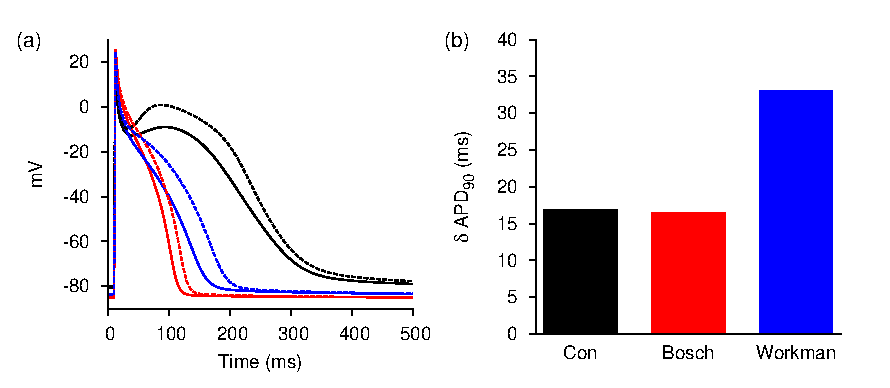
\includegraphics{figures/toolkit/afer/figures/01_APD}
\caption[AFER AP Plots And APD differences]{
\label{fig:toolkit:afer:apd}
(a).
Action potential profiles after pacing at \unit{1}{Hz}.
Results are shown for AM/PM cells (solid lines) and CT cells (dashed lines).
Control parameter traces are black, Bosch are red and Workman traces
blue.
The CT cells have a longer APD in all cases and show an elevated plateau
potential.
(b).
APD differences between AM/PM cells and CT cells after pacing at \unit{1}{Hz}.
Colour scheme as for panel (a).
There is almost no difference in $\delta$\apd\ between control and Bosch CT cells,
but $\delta$\apd\ increased markedly when Workman parameters are used.
}
\end{figure}

Incorporating the heterogeneity and AFER data causes significant differences in
\apd\ and AP morphology to manifest, as shown in
figure~\ref{fig:toolkit:afer:apd}(a).
The effects of AFER are not uniform across the different cell types of the
atrium in both cases (figure~\ref{fig:toolkit:afer:apd}(b)).
The difference in the AP between AM/PM myocytes and CT myocytes in the Workman
remodelled case is almost double that seen in either the Bosch remodelled case
or control case.
Note that in all cases there is almost no difference between AM and PM types.


\begin{figure}
\centering
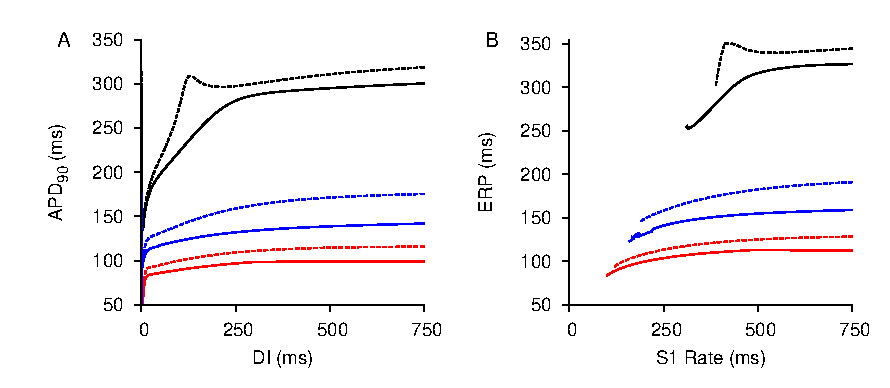
\includegraphics{figures/toolkit/afer/figures/02_APDR}
\caption[AFER APDr and ERPr curves]{
\label{fig:toolkit:afer:apdr}
(a)
\apdr\ curves showing \apd\ plotted against diastolic interval (DI) for control
(black), Bosch (red) and Workman (blue) cases.
AP/PM curves are shown as solid lines, CT curves are dashed.
AFER acts to flatten the restitution curves.
In all cases CT \apd\ is above AM/PM \apd.
(b)
ERP\emph{r}\ curves showing ERP plotted against S1 interval.
Colour scheme is as for panel (a).
In all cases CT ERP is above AM/PM ERP.
Note that AFER enables successful excitation at much lower S1 intervals.
}
\end{figure}

The \apdr\ curves, shown in figure~\ref{fig:toolkit:afer:apdr}(a), are
flatter over much of the range of diastolic intervals for Bosch and Workman as
compared to control.
The curves have two clear phases in the AFER cases; a very steep initial rise
and then slower, asymptotic rise in \apd.
In the control case the curves show an intermediate a phase with a slope between
the two extremes.
In the control CT case, the curves include a prominent notch at a DI of
approximately \ms{130}\ which is caused by the up regulation of \ii{Ca,L}\ in CT
cells.
The down regulation associated with the AFER removes this.
In both of the AFER cases, the curves are almost flat at DI \ms{750}, but in the
control case, the \apd\ is still rising.
The figure also emphasises the increased heterogeneity observed in the Workman
case.

In AF tissue, the ERP\emph{r} was flattened for all tissue types compared with
the control cells, as shown in figure~\ref{fig:toolkit:afer:apdr}(b).
The curves also extended to lower S1 intervals for AF tissue, indicating that it
was possible to excite AF tissue successfully at a higher rate than was possible
in control tissue.
Heterogeneity in ERP\emph{r} was largely unaffected by AF.

\begin{figure}
\centering
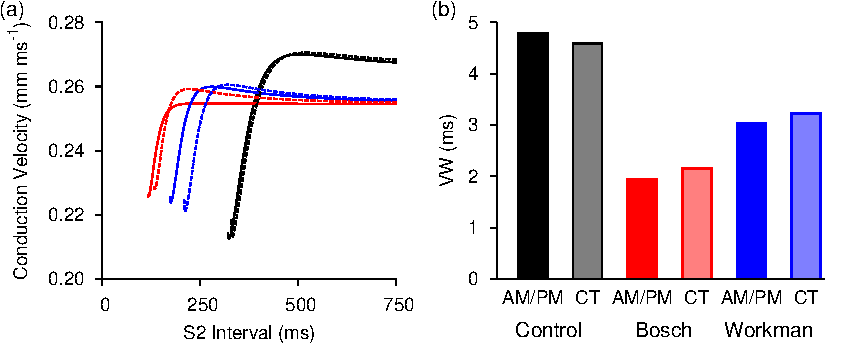
\includegraphics{figures/toolkit/afer/figures/03_CVR}
\caption[AFER CVr curves and VWs]{
\label{fig:toolkit:afer:cvr}
(a) 
CV\emph{r}\ curves for Control (black), Bosch (red) and Workman (blue) tissues.
AM/PM cells are indicated by solid lines, CT cells by dashed.
In all cases CT cells show a higher conduction velocity at long
($>$\ms{600}) S2 intervals, but AM/PM muscles allow faster conduction at lower
S2 intervals.
AF cases show a reduced CV in all instances and support
higher pacing rates via reduced minimal interval.
(b) Vulnerability Window for Control (black), Bosch (red) and Workman (blue).
AM/PM cell types are shown solid, CT are partially shaded.
The VW is reduced for the AF remodelled cases via reduced excitability.
The presence of the remodelling also reverses the difference in VW between cell
types.
}
\end{figure}

Conduction velocity, shown in figure~\ref{fig:toolkit:afer:cvr}(a), was slowed by AF,
reducing the solitary wave velocity from $0.27\,\text{mm}\,\text{ms}^{\text{-1}}$\ in
control to $0.25\,\text{mm}\,\text{ms}^{\text{-1}}$\ in Bosch and
$0.26\,\text{mm}\,\text{ms}^{\text{-1}}$\ in
Workman.
Maximal pacing rate increased from the control value of \unit{187}{bpm} to
\unit{512}{bpm} in Bosch strands and \unit{347}{bpm} in Workman strands of AM or
PM cells.
In CT strands, maximal pacing rates of \unit{183}{bpm}, \unit{451}{bpm}\ and
\unit{287}{bpm}\ were observed for Control, Bosch and Workman cases
respectively.
The heterogeneity of minimal pacing intervals is significantly increased by
AFER, from \unit{4}{bpm}\ to over \unit{50}{bpm}\ in Bosch and Workman strands.

The VW was reduced by AF, figure~\ref{fig:toolkit:afer:cvr}(b).
The control value of \ms{4.8}\ was reduced to \ms{2.0}\ in Bosch and \ms{3.0}\ in Workman for AM and PM cell types.
In CT cells under control conditions, the VW was reduced to \ms{}
The reduction in VW for CT cells was reduced, to \ms{4.6}.
In contrast, the VW increased for AF cases; \ms{2.1}\ and \ms{3.2}\ for Bosch
and Workman cases respectively.


\begin{figure}
\centering
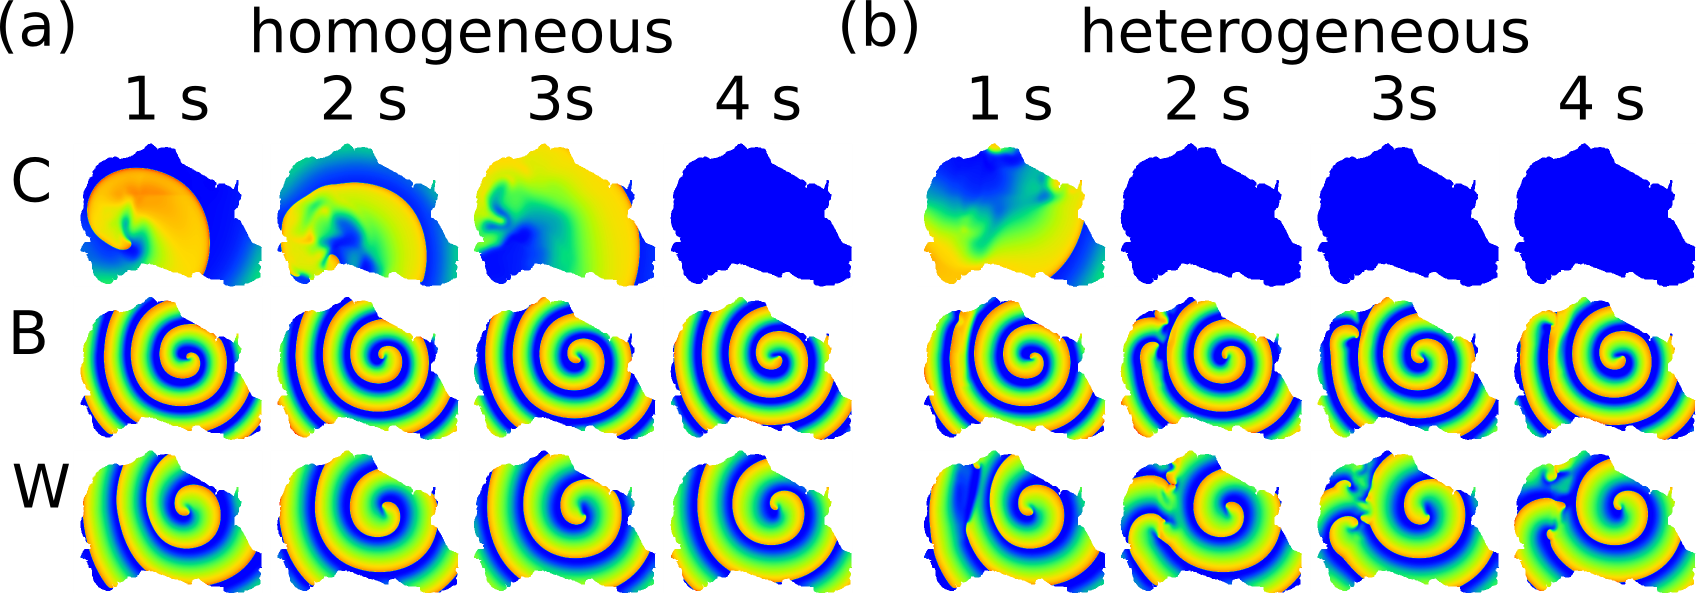
\includegraphics{figures/toolkit/afer/2d_plots}
\caption[AFER 2D re-entry plots]{
\label{fig:toolkit:afer:2d}
Simulation of re-entry in 2D sheets of electrically homogeneous
(a) and electrically heterogeneous (b) sheets.
Colour represents membrane potential from blue (resting) to orange (excited).
Columns show representative frames after initiation of re-entry at t = 0.
Rows C, B, W show data from control, Bosch and Workman cases, respectively.
Re-entry self-terminated under control conditions in both homogeneous (a)(C) and
heterogeneous (a)(C).
Under AF conditions, re-entry becomes a sustained mother rotor in
electrically homogeneous conditions ((a)(B), (a)(W)).
However, under electrically heterogeneous conditions AF causes re-entry to degenerate
into erratic propagations on the borders of the heterogeneity ((b)(B), (b)(W)) }
\end{figure}

Simulations over the 2D geometry examined the lifetime and behaviour of
spiral waves in the presence and absence of electrical heterogeneity.
As can be seen in figure~\ref{fig:toolkit:afer:2d}, panels (a)(C) and (b)(C), re-entrant
activity self-terminated in both homogeneous and heterogeneous cases.
Spiral wave meander over a large region of tissue eventually causes the tip to
leave the tissue.
Self-termination was much more rapid in the electrically heterogeneous case,
taking \unit{1.31}{s}, compared with \unit{3.20}{s} in the homogeneous case.

Conversely, under AF conditions the re-entry persisted after it was
induced for the whole period of the simulation, a lifespan of over \unit{5}{s}.
Under electrically homogeneous conditions, panels (a)(B) and (a)(W) show a
stable mother rotor rotating anti-clockwise in the tissue.
In heterogeneous conditions, as shown in panels (b)(B) and (b)(W), a similar
mother rotor to the homogeneous cases is visible towards the right of each
frame.
On the left of the frames, the rotor breaks up into multiple fibrillatory
wavelets on the border of the heterogeneous regions, forming a complex and
chaotic pattern of excitation.


\subsection{Discussion and conclusions}

AFER induces significant changes in the cellular electrophysiology that
appear to affect rate dependent electrical activities.  It helps to
sustain re-entry, providing evidence to substantiate the hypothesis of
`AF begets AF'.

The single cell results show a striking reduction in the \apd\ and
repolarization properties.
AFER abbreviated \apd\ in AM cells by 66~\% in Bosch and 53~\% in Workman.
Other work~\cite{Xie2002,ByungSoo2002,Karma1994,Tusscher2006} has already suggested why flattening of
the ERP and APD restitution curves can be pro-arrhythmogenic.
Our study suggested that reduction is not uniform across all cell types, which
leads to an augmented heterogeneity.

From the 1D results, AFER tissue forms a much better substrate for arrhythmic
activity.
It supports a much higher pacing rate and has a reduced conduction wavelength
(conduction velocity multiplied by \apd), allowing a greater number of
excitation waves to exist in the tissue.
The increase in the heterogeneity of the maximal pacing rates suggests that
remodelled tissues might be more vulnerable to localised regions of conduction
block.
This has been shown to lead to re-entry~\cite{Xie2001a}.

The 2D simulations in the realistic sheet show a marked difference in
re-entrant behavior between homogeneous and heterogeneous simulations.
The homogeneous sheets show self-termination of re-entry in control
tissue, whilst the reduced ERP and conduction wavelength allow the rotor
to remain stable and persist for the duration of the simulation in AFER
condtions as is expected from the flattened restitution
curves~\cite{Xie2002,Karma1994}.
The heterogeneous sheet simulations, show spiral wave
breakup, as observed in real tissue \cite{Kumagai1997}, in both control
and AF simulations, possibly due to elevated plateau potentials and
increased refractory period of the CT cells~\cite{Clayton2005}, combined with
the slower conduction velocity at high pacing rates.
Self-termination is still observed in control simulations and is more rapid than
in homogeneous tissue.

It is still unclear about the pro- or anti-arrhythmogenic effects of
electrical heterogeneity in the human atria.  Self-termination is more
rapid in the heterogeneous tissue for the control case, but despite AFER
increasing the heterogeneity between tissue types, it doesn't lead to
self termination of the re-entry.  In fact, it leads to breakup of the
spiral wave in the region of the heterogeneity, leading to a region of
erratic propagations, as has been seen in experiment~\cite{Kumagai1997}.
Further study, in both 3D geometries and physiological experiments,
would be needed to elucidate the true effects of the heterogeneity.


\section{Anion Currents In The Human Atrium}

In a recent experimental study, Li et al.~\cite{Li2007} determined the existence
of a novel outwardly rectifying anion current in human atrial myocytes isolated
from right atrial appendages taken from patients undergoing coronary bypass
surgery.
Unlike previously observed chlorine bearing
currents (e.g.~\cite{Sorota1992,Kawano1995,Harvey1989a}), the new current is
basally active.
It does not respond to changes in cell shrinkage or the stilbene diphosphonate
$\text{Cl}^{\text{-}}$ channel blocker.
This could represent a new target for anti-arrhythmic drugs, but there are no
highly selective modifiers of the current currently known.
This makes computational modelling of the current attractive.

A preliminary computational study has been conducted~\cite{Li2007}\ to
investigate the effects of the anion sensitive current, \ii{ANION}, on atrial
action potentials.
However it is still unclear on how this novel current affects intercellular
excitation conduction and cellular restitution properties.
It was known from the Li et al. study that influence on the atrial AP was small.
This study extended that to restitution properties and intercellular excitation
conduction.
It was expected that a small current would have a small influence on such
properties.
This would then have a small influence on the behaviour of spiral waves in two
dimensions.

\subsection{Methods}

The Li et al.~\cite{Li2007}\ study determined the current carried by this novel
ion channel, \ii{ANION}, could be modelled by
\begin{equation}
\label{eqn:anion:ianion}
I_{ANION} = g_{ANION} \frac{V-E_{ANION}}{1-\left(c\times e^{d\times\left(V-E_{ANION}\right)}\right)}
\end{equation}
where $g_{ANION}$ is the conductivity of the anion channel, $E_{ANION}$ is
the reversal potential of the channel and $c$ and $d$ are constants to
describe the behaviour.
All other symbols have their usual meanings.
They presented two sets of parameters for (\ref{eqn:anion:ianion}) given in
table~\ref{tbl:anion:params}, which described the current through the channel
when carrying a majority of \nothree\ or $\text{Cl}^{\text{-}}$ ions.

\begin{table}
    \caption[Parameter sets for the anion carrying current]{
        Parameter sets for the anion sensitive current \ii{ANION}\ when carrying
        \nothree\ and $\text{Cl}^{\text{-}}$\ ions.
    }
    \begin{center}
    \begin{tabular}{ l  c c}
    \toprule
    & \nothree & $\text{Cl}^{\text{-}}$ \\
    \midrule
    $g_{ANION}$ & 0.37   & 0.19 \\
    $E_{ANION}$ & -45.64 & -45.64 \\
    $c$         & 0.87   & 0.94 \\
    $d$         & $8.4\,\text{x}\,10^{\text{-4}}$ & $2.5\,\text{x}\,10^{\text{-4}}$\\
    \bottomrule
    \label{tbl:anion:params}
    \end{tabular}
    \end{center}
\end{table}

This simulation study used the parameter set for the anion current carrying
$\text{Cl}^{\text{-}}$ ions.
The effects of the addition of this current to atrial myocyte cells was
quantified.
In the following paragraphs, `control' is used to denote the original
Courtemanche~et~al.~\cite{CRN98}\ atrial myocyte model and `anion' to denote the
Courtemanche~et~al. model with the addition current described by
(\ref{eqn:anion:ianion}) and using the $\text{Cl}^{\text{-}}$ parameter set from
table~\ref{tbl:anion:params}.

The effect on the behaviour of the cells caused by the anion current was
quantified using the simulation library described in
chapter~\ref{chapter:toolkit}\ for
control and anion cases.
As this simulation study was based on the CRN cell, the standard stimulus was
\ms{2} in duration and \unit{2}{nS} in magnitude.
Unless an alternative protocol is mentioned, all simulations directly followed
those described in Section~\ref{sec:toolkit:protocols}.

Simulating a single cell, the following measures were quantified: the AP
profile, the restitution of APD at 50\% repolarization, \apdr[50], the
restitution of APD at 90\% of repolarization, \apdr\ and the Effective
Refractory Period restitution, ERP\emph{r}.  The maximal fast sodium activation
was quantified at the same time as the \apdr\ was computed and is the product of
the three gates in \ii{Na}, as $m^{3}hj$. In all the single cell cases, the
cell was paced 10 times before the measurement was taken, to allow simulation
parameters to settle and to adapt to any changes in pacing rate.  Storage of the
cellular state was used in all appropriate points in the simulation, to minimise
computational time.

Using a 1D strand model the temporal Vulnerability Window to unidirectional
conduction block, VW, the Conduction Velocity restitution, CV\emph{r}\ and the
threshold of excitation were computed.  The strand model used was 300 nodes long
and had a space step of \mm{0.1}.  The diffusion coefficient, $D$, was set to
$0.03125\,\text{mm}^{\text{2}}\,\text{ms}^{\text{-1}}$~\cite{Biktasheva2005}.
In all 1D simulations the strand was paced 10 times before measurement was
taken.  In all simulations this state was then cached and restored as
appropriate, as described in the algorithms section of this chapter.

Using a 2D tissue model the lifetime of re-entrant spiral waves was estimated,
following the wave-break protocol outlined earlier.  The sheet had dimensions of
$375\times375$ nodes and a space step of \mm{0.1}.  The clamp potential used
to break the wave was \mv{0} and it was applied for \ms{1}.

\subsection{Results}


\begin{figure}
\begin{center}
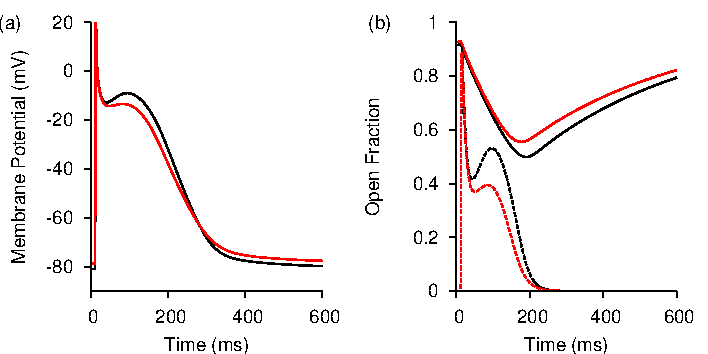
\includegraphics{figures/toolkit/anion/figures/01_AP}
\end{center}
\caption[Anion Current AP Profiles and \ii{Ca,L}\ gating parameters]{
\label{fig:tookit:anion:ap}
(a) AP profile for the CRN model in control (black) and anion (red) cases.
The inclusion of the $\text{Cl}^{\text{-}}$ carrying current results in a small
change of AP morphology, with a depressed plateau potential and an elevated
resting potential.
(b) Fractional opening of the gates of \ii{Ca,L}.
The $d$ (activation) gate is shown dashed, the $f$ (inactivation) gate solid.
Colours as in panel (a).
The $f$ gate takes longer to inactivate, whilst the $d$ gate does not activate
as much.
}
\end{figure}

The AP generated by the control and anion simulations are shown in
figure~\ref{fig:tookit:anion:ap}(a).
The \apd\ is slightly reduced from \ms{299.6} to \ms{297.3}, whereas the
\apd[50]\ is more significantly reduced, from \ms{180.1} to \ms{158.1}.
The AP profile shows a depressed plateau region (phase 2), reduced from
\mv{-9.56}\ to \mv{-14.1}\ and a slightly elevated resting potential,
\mv{-79.0}\ in the anion case cf. \mv{-80.9}\ in control.
This is consistent with the Li~et~al.~\cite{Li2007} study, and is included here
only for completeness.

Transients of the $d$ and $f$ gate of the \ii{Ca,L}\ open fractions are shown in
figure~\ref{fig:tookit:anion:ap}(b).
The $f$ gate in the \ii{ANION}\ case has a higher fraction of open channels for
longer than the control case.
The $d$ gate does not activate as much in the plateau region, contributing to
the shorter plateau.


\begin{table}
\caption[Calculated parameters for anion and control cells]{
\label{tbl:toolkit:anion_params}
Various calculated parameters for control (original CRN cell) and anion (CRN
cell modified to include $\text{Cl}^{\text{-}}$-carrying current).
The duration of the action potential at 50\% and 90\%
repolarization, \apd[50]\ and \apd\ respectively.
The maximum observed upstroke velocity of the action potential,
$\frac{dV}{dt}_{max}$.
The temporal vulnerability window to unidirectional conduction block, VW.
}
\begin{center}
\begin{tabular}{r l l l l}
\toprule
Case & \apd\ (ms) & \apd[50]\ (ms) & $\frac{dV}{dt}_{max}$ ($\text{mV}\,\text{ms}^{\text{-1}}$) & VW (ms)  \\
\midrule
Control & 299.6 & 180.1 & 217.1 & 3.22 \\
Anion & 297.3 & 158.1 & 210.6 & 3.94 \\
\bottomrule
\end{tabular}
\end{center}
\end{table}

The computed APD\emph{r}\ curves under the control and anion conditions are shown
in figure~\ref{fig:tookit:anion:apdr}(a) and \ref{fig:tookit:anion:apdr}(b), for the
restitution curves of APD at 50\% (\apdr[50]) and 90\% (\apdr) of repolarization,
respectively.
The
\apdr[50]\ shows the most significant differences, with the anion
curve depressed by \ms{20} even at the largest DI, increasing to a maximum
difference of over \ms{40} at at DI of \ms{380}.
The two curves then cross over at a DI of \ms{200}.
The \apdr\ curves, by contrast, are very similar for control and anion cases at
large (over \ms{600}) DI.
Between \msrange{100}{400}\ DI, the anion case is depressed compared to the control
case, with a difference of up to \ms{25}\ observed in the measured APDs.  At
\ms{100}, the curves rejoin one another and show a rapidly increasing slope as the
DI approaches \ms{0}.

\begin{figure}
\begin{center}
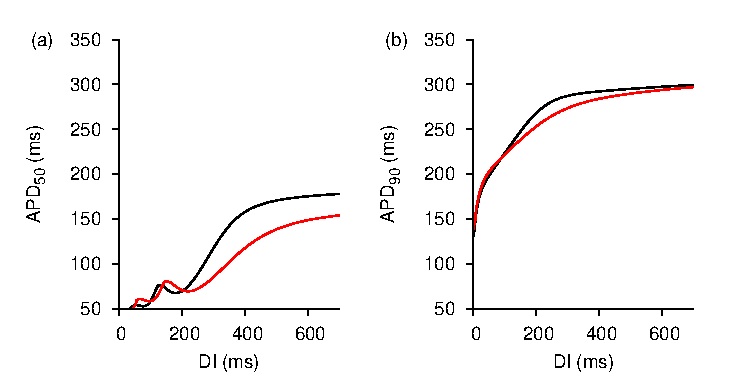
\includegraphics{figures/toolkit/anion/figures/02_APDR}
\end{center}
\caption[Anion Current APD Restitution]{
\label{fig:tookit:anion:apdr}
(a)
\apdr[50] curves for the CRN model in control (black) and anion (red) cases.
The two variants are different for all the DI in the simulation,
with the anion case below the control case for much of the DIs.
The slope is reduced by \ii{ANION}, compared to
the control case.  The curves cross at DI \ms{200}.
(b)
\apdr curves for the CRN model in control and anion cases.
The two variants behave the same at large DIs, but at decreasing DI the
anion case shows a greater reduction in the \apd.
At short DI (below \ms{100}) the two curves rejoin each other.
}
\end{figure}
\begin{figure}
\begin{center}
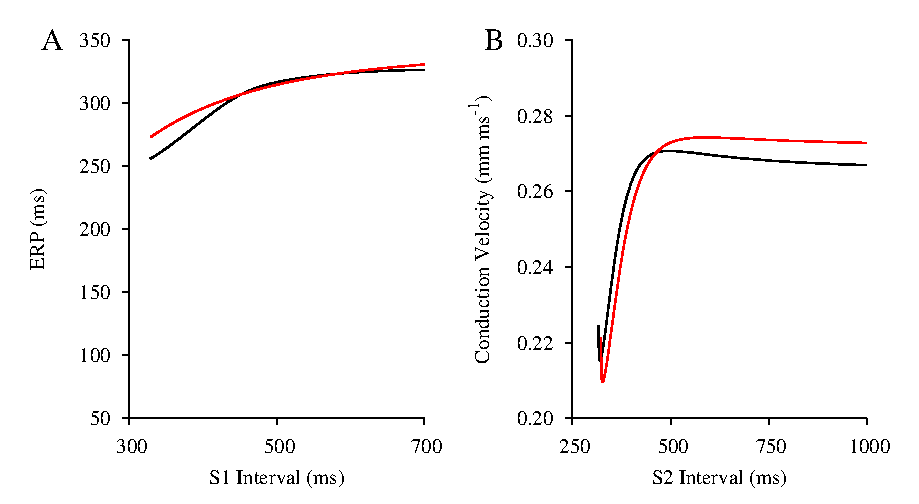
\includegraphics{figures/toolkit/anion/figures/03_ERPR}
\end{center}
\caption[Anion Current ERPr and CVr] {
\label{fig:toolkit:anion:erpr}
(a)
ERP\emph{r} curves for the CRN model in control (black) and anion
(red) cases.
The addition of the \ii{ANION} current changes the behaviour of the cell from a long
and flat plateau region followed by a relatively sharp decrease into a more
constant decline.
(b)
CV\emph{r}\ curves for the CRN model in control and anion cases.
 The CV\emph{r}\ curves are relatively flat for both cases over the range of
\msrange{500}{1000}, before they decrease rapidly in CV until the minimum
S2 interval is reached at approximately \ms{320}.
The CV is higher for the anion case at longer S2 intervals, before it
falls below control at an approximate S2 interval of \ms{460}.
}
\end{figure}

The ERP\emph{r} curves produced by the control and anion cases are shown in
figure~\ref{fig:toolkit:anion:erpr}(a).
In both cases the ERP\emph{r}\ curves are relatively
flat, decreasing by approximately \ms{60}\ over the \ms{700}\ range of S1
intervals considered.  The addition of the \ii{ANION}\ current changes the
behaviour of the ERP\emph{r} curve in a manner which is not simply a shift left
or right.  The control case shows a response which has a clear plateau region
which continues until an S1 interval of \ms{500}\ is reached and then a
relatively steeper decline until eliciting an AP of the appropriate magnitude
becomes impossible at an S1 interval of \ms{330}.  The anion case, by contrast,
shows a decreasing ERP over the whole range of S1 intervals considered although
it too shows its steepest slope just before eliciting a sufficiently large AP
becomes impossible, also at approximately \ms{330}.  At long S1 intervals (above
\ms{700}) the ERP\emph{r}\ is longer for the anion case before the curves cross
at \ms{600}\  and then again at \ms{450}\ with the ERP in anion at the point
where further stimulation becomes impossible almost \ms{20}\ higher than in the
control case.

The temporal VW increased with the addition of the anion current from \ms{3.22}
in control to \ms{3.94}\ in anion case, a 22\% increase in the size of the
region of unidirectional conduction block, shown in table~\ref{tbl:toolkit:anion_params}.
The CV\emph{r}\ curves, shown in
figure~\ref{fig:toolkit:anion:erpr}(b), suggest that tissue with the anion sensitive current
shows faster CV at normal physiological stimulus intervals (corresponding to
\msrange{500}{1000}).
The average conduction velocity with \ii{ANION}\ is
$0.274\,\text{mm}\,\text{ms}^{\text{-1}}$ in anion,
compared with $0.268\,\text{mm}\,\text{ms}^{\text{-1}}$ in control in this range
of S2 intervals.
As the conduction interval is reduced below \ms{500}, the conduction velocity
starts to decrease rapidly until conduction stops at \ms{323.4} for anion and
\ms{317.1} for control.
There is a brief recovery of conduction velocity visible in both cases, just
before conduction block.

\begin{figure}
\begin{center}
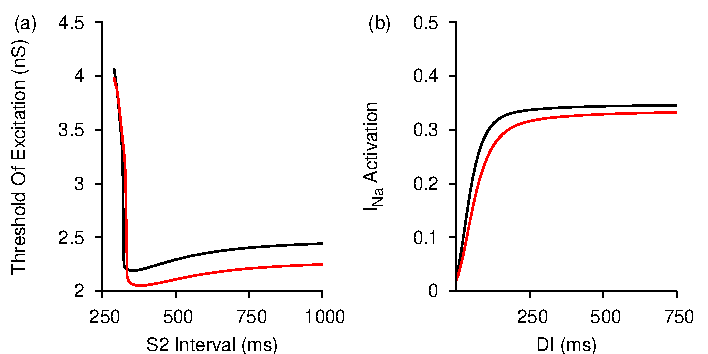
\includegraphics{figures/toolkit/anion/figures/04_ToE}
\end{center}
\caption[Anion Sensitive Threshold Of Excitation and \ii{Na} activation]{
\label{fig:toolkit:anion:toe}
(a)
Threshold of excitation curves in control (black) and
anion (red) cases.
As S2 decreases, so does the threshold of excitation until a critical point is
reached and the current which must be injected to reach the threshold almost
doubles.
In the control this comes at a $\Delta t$ of
\ms{321}\ and in anion at \ms{330}.
Until the critical point threshold of excitation is consistently lower for cells
with \ii{ANION}\ present.
(b)
Maximal activation of the fast sodium current, \ii{Na}, as DI is decreased.
The fast sodium current consistently activates to a greater degree in control
cases.
The effect is rate dependent with the greatest difference observed at DI \msrange{150}{200}.
}
\end{figure}

The threshold of excitation, shown in figure~\ref{fig:toolkit:anion:toe}(a), shows that
\ii{ANION} reduces the minimum stimulus current by approximately \unit{0.2}{nS},
a reduction of 10\%, at almost all $\Delta t$\ intervals.  It is also
interesting to note that both control and anion tissue types show `supra-normal'
excitability, with the minimum stimulus current decreasing as $\Delta t$\
decreases.  This occurs until a critical point is reached when the cell suddenly
becomes significantly harder to excite, with the minimum stimulus current
increasing almost 100\%.
This occurs \ms{9}\ later in control tissue at
\ms{321}\, compared with \ms{330}\ in control.

The maximal activation of the fast sodium current, \ii{Na}, is shown in
figure~\ref{fig:toolkit:anion:toe}(b).
The presence of \ii{ANION}\ consistently reduces the maximal activation of \ii{Na}.
At long DI, greater than \ms{400}, the reduction is 3\%, increasing to almost
twice that in the range of \msrange{150}{200}.
Both curves rapidly decrease to almost no \ii{Na}\ activation at an DI of
\ms{0}\ but the anion case starts this descent first.
\begin{figure}
\begin{center}
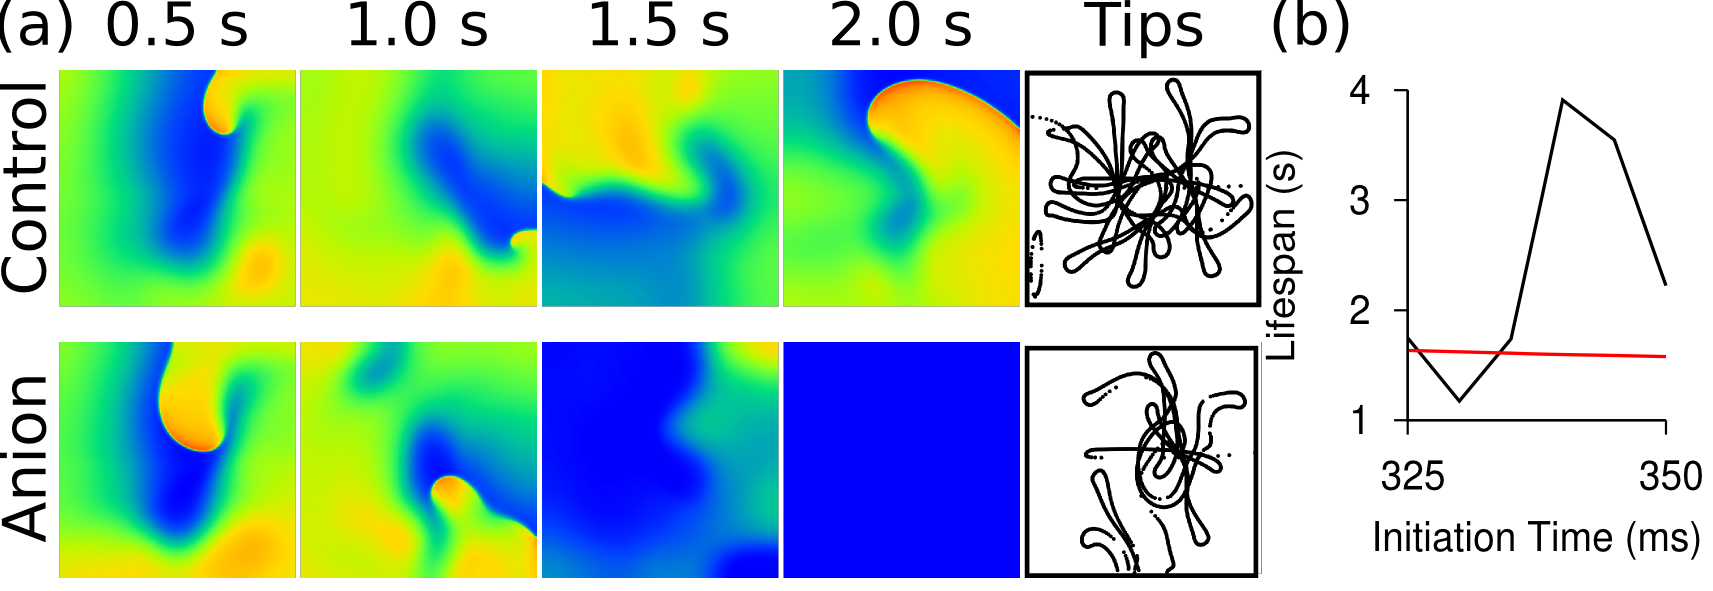
\includegraphics{figures/toolkit/anion/twod_traces}
\end{center}
\caption[Anion Sensitive Tissue Sheets and Spiral Lifespans]{
\label{fig:toolkit:anion:spiral}
(a)
Representative membrane potentials and tip trace for control (top row) and anion
sensitive cases (bottom row).
Times are from the initiation of spiral activity via cross--field protocol.
Cross--field stimulus was delivered at \ms{345}\ wall time.
Colour represents membrane potential and is coloured from blue (depolarised,
\mv{-80}) to orange (excited, $>\mv{0}$).
Both spiral waves are highly mobile, meandering over a very large area of
tissue.
(b)
Lifespan as related to time of initiation.
Lifespan in \ii{ANION}\ is relatively constant at around \ms{1600}\ whilst
control lifespan fluctuates considerably.
}
\end{figure}
Spiral waves were induced in a square sheet.
Representative plots of the
membrane potential over the whole sheet, produced as the simulation was ongoing,
are shown in figure~\ref{fig:toolkit:anion:spiral}(a).
The top row corresponds to control tissue, whilst the bottom row has an
\ii{ANION}\ sensitive current active.
Times of the membrane potential snapshots are relative to initiation of reentry at t = \ms{345}.
Tip traces are in the 5th column.
In both cases the spiral wave starts in the centre of the tissue and then follows a
looping track around the tissue before finally it exits the tissue when it
cannot turn fast enough around its own refractory tail.
Lifespans of reentry from differing initiation times are shown in
~\ref{fig:toolkit:anion:spiral}(b).
Lifespan in \ii{ANION}\ is relatively constant at around \ms{1600}\ whilst
control lifespan fluctuates considerably, from \ms{1175}\ to \ms{3910}.

\subsection{Discussions and Conclusions}

The effects of the inclusion of an anion sensitive current do not seem to be
that large, at least when considered on the single cell level.
However, despite the small influence of the current on the action potential duration,
it does have noticeable effects on the restitution properties of the cell and
on the behaviour of cells in a tissue.
The general behaviours of the Courtemanche cell have been discussed elsewhere,
for example in~\cite{CRN98,Cherry2008a}, I only discuss the differences the
\ii{ANION}\ current makes.

The most noticeable effect of the inclusion of \ii{ANION}\ in a cellular model
is the abbreviation of the \apd[50]\ and an accompanying reduction in the
plateau potential.  The abbreviation is due to \ii{ANION}\ acting as a
rectifying current when the membrane potential is above \mv{-45}.   Conversely,
at potentials below \mv{-45}\ \ii{ANION}\ acts to depolarize the cell, leading
to the slightly elevated resting membrane potential observed between action
potentials.  This difference in effect is what leads to the interesting
behaviours observed in cells with \ii{ANION}.

The \apdr[50]\ and \apdr\ curves show that \ii{ANION} has a rate dependent
effect.  Both curves are flattened in the cells which include \ii{ANION}\, but
this flattening is not uniform over the range of DIs considered.
\ii{ANION}\ has a simple exponential dependence on the membrane potential and no
time-dependent gating variables however, so it is not \ii{ANION}\ that causes
this rate dependence directly.
Instead, we must look to the currents active within the plateau region of the
action potential.
\ii{CaL}\ is the principle current responsible for the plateau region of the
action potential and unlike \ii{ANION} it has both time and voltage dependant
gating variables for activation, $d$, and inactivation, $f$.
The $d$\ gate is not as interesting as the $f$\ gate, as its time-course is not
affected by the presence of \ii{ANION}, although its activation during the
plateau region is reduced.
However, the $f$\ gate in \ii{ANION} cells never inactivates as completely as
it does in the control simulations which lack the current.

For the 1D strand results, both the CV\emph{r} and threshold of
excitation data also show rate dependent influence.
At a long stimulus interval, the increased excitability of the cell by the anion
current leads to a higher conduction velocity~\cite{Nygren2000}.
The increased excitability at long stimulus interval is due to the inward nature
of the anion current in the very first stages of the action potential.
This increased excitability allows atrial cells with \ii{ANION}\ to conduct the
excitation wave faster until, when the stimulus interval reaches a critical value of
\ms{500}, control cells start to conduct faster.
At this stimulus interval, the threshold of excitation is still lower for the
anion case, so another factor is responsible for the reduction in conduction
velocity.
The excitability of the cell is an important influence on the conduction
velocity, but it is not the only factor.
Another major factor is the upstroke velocity of the action potential which is principally
determined by the fast sodium current, \ii{Na}.
This is partially inactivated by the elevated resting potential in the anion
case, which also reduces the rate of recovery of the inactivation variables.
When the test stimulus is delivered after a reduced conduction interval in the
anion case \ii{Na}\ does not open as fully, slowing the upstroke and thus
leading to a reduced conduction velocity at short stimulus intervals, compared
with the control case.

The increase in the
vulnerability window appears to be quite significant, at over 20\% larger than
the vulnerability window in tissue without \ii{ANION}.
An increased vulnerability window has an obvious influence on the genesis of
re-entrant excitation---A larger vulnerability window increases the chance of a
premature excitation interrupting the normal function of the heart.
Though in both cases, the vulnerability window is relatively small.


Dynamic behaviours of the 2D spiral wave are interesting.
Both cells show a highly mobile spiral tip, due to their long \apd\ and ERP
relative to the size of the tissue.
However in the \ii{ANION}\ case, this does not translate into a widely varying
spiral lifespan, as might be expected from such mobility.
The restitution properties are generally slightly flattened by the inclusion of
\ii{ANION}, although perhaps importantly here, in the rapid pacing region, the
ERP is higher for \ii{ANION}\ bearing cells.
Further investigation, perhaps using the phase field
method~\cite{Biktashev1994}\ to start with a `stationary' spiral would be of use
to elucidate the effects.


\section{Modelling the Whole Atrium: Conclusion}

A realistic model of the human atria has been developed.
The model uses a biophysically detailed second generation cellular
electrophysiological model to describe the action potential kinetics at each node.
The model includes a simplistic but effective electrophysiological
heterogeneity, in the absence of more detailed experimental data.
Solution times for the model are improved by the use of lookup tables for
voltage dependent values.
The geometry is based on data from a real human dataset.
A simple description of fibre orientation has been included and conduction
anisotropy has been considered.
The resulting whole atrium model has a good parallel fraction and is solvable in
tractable times on modern hardware.

The model accurately reproduces the activation sequence of the healthy human
atrium.
Time to total activation and individual tissue conduction velocities both fall
within experimental and clinical values.
Thanks to the use of a biophysically detailed model of cellular action
potential, the model can also be used to simulate pathological cases such as
familial atrial fibrillation.

The S140G mutation in the KCNQ1 protein causes a dramatic change in the
electrophysiological behaviours of the \ii{Ks}\ rectifier current.
The up-regulation of the \ii{Ks}\ channel causes a large reduction in the \apd.
This then influences the rest of the electrophysiology, effecting all aspects of
the cellular electrical behaviour.
It is very easy to see how the mutation is associated with a prevalence of
atrial fibrillation in families which have inherited the gene.

The AFER study, by contrast, involved remodelling where many currents were
affected.
In this study, the restitution curves were significantly flattened, leading to
stable spiral waves.
Regional differences in AP profiles, caused by the natural heterogeneity of the
atrium, lead to breakup on the edges of such regions.

In the \ii{ANION}\ study, the influence of a novel anion bearing current in the
human atrium was examined.
Despite the small influence of the current on the \apd\ and its time independent
nature, there were significant alterations in the rate dependant and dynamic
behaviours of the cell.
This is due to the voltage at which the current act, and the corresponding
alterations to the time courses of currents which do have time dependent
properties.

All three experimental studies involved the use of the toolkit developed in
chapter~\ref{chapter:toolkit}.
They showcase its versatility in modelling effects from the subtle, such as
\ii{ANION}, to severe, such as the S140G mutation study.
In addition, the S140G study demonstrates (a reduced version of) the whole
atrium model in operation.
